%  PREAMBULO %%%%%%%%%%%%%%%%%%%%%%%%%%%%%%%%%%%%%%
% ------------------------------------------------
%          FILE:  como-aprender-ingles.tex
%       CREATED:  Dom 30/Dez/2012 hs 15:45
%   LAST CHANGE:  2013 Mar 25 09:05:24 AM
%        AUTHOR:  Sérgio Luiz Araújo Silva
%          SITE:  http://vivaotux.blogspot.com
%       TWITTER:  @voyeg3r
%         SKYPE:  sergioaraujosilva
% -------------------------------------------------
\documentclass[a4paper,12pt,openany,]{book}
\usepackage[utf8x]{inputenc}
\usepackage[portuguese,brazil]{babel}
\usepackage{setspace}
\usepackage{makeidx}    % para gerar o índice remissivo
\usepackage{graphicx,color}   % \includegraphics[opt=valor]{figura.png} \textcolor{red}{texto em vermelho}
\graphicspath{{./img/}}
\usepackage{verbatim}   % para algoritmos
\usepackage{color}      % use if color is used in text
\usepackage{subfigure}  % use for side-by-side figures
\usepackage{url}        % para usar url's :)
\usepackage{pifont}	    % simbolos de setas
\usepackage{enumitem}   % tentando diminuir o espaçamento entre itens no itemize
\usepackage{multicol}   % criar texto em colunas
%\usepackage{verbatin}	% inserir códigos fonte
\usepackage{flafter}    % make sure figures do not appear before their text:
\frenchspacing          % não trata etc. como fim de senteças
\usepackage{xcolor}     % para usar cores no documento
\definecolor{bl}{rgb}{0.0,0.2,0.6}
\usepackage{cmap}  % para mapear caracteres especiais no pdf
\usepackage[pdftex]{hyperref}  % suporte a hypertexto e links
\usepackage{lastpage}  % mostra o número da última página

% para gerar o pdf use:  pdflatex text.tex

% fonte garamond
%\usepackage[urw-garamond]{mathdesign}
%\usepackage[cardo]{mathdesign}
\usepackage{inconsolata} % para comandos
% fonte libertine
\usepackage{libertine}
\usepackage[T1]{fontenc}

% fonte palatino
%\usepackage[sc]{mathpazo}
%\linespread{1.05}         % Palatino needs more leading (space between lines)
%\usepackage[T1]{fontenc}

\makeindex
\newcommand{\dica}[1]{{{\large \ding{42}}}}	% inserir imagem para dica, provido por pifont

\hypersetup{colorlinks=true, breaklinks=true, linkcolor=blue, citecolor=blue, filecolor=blue, pagecolor=blue, urlcolor=blue,
%\hypersetup{colorlinks=false,pdfborder={0 0 0},breaklinks=true}
pdfauthor={anonymous},
pdftitle={How to learn english easily},
pdfsubject={english},
pdfkeywords={english, ingles},
pdfproducer={Latex},
pdfcreator={pdflatex}}

\usepackage{fancyhdr} % para cabeçalhos mais elaborados
\pagestyle{fancy}
% com isto nos nos certificamos que o cabeçalho dos capítulos e
% seções estão em minúsculo.
\renewcommand{\chaptermark}[1]{\markboth{#1}{}}
\renewcommand{\sectionmark}[1]{\markright{\thesection\ #1}}
\fancyhf{} % deleta a configuração atual para cabeçalho e rodapé
\fancyhead[LE,RO]{\bfseries\thepage}
\fancyhead[LO]{\bfseries\rightmark}
\fancyhead[RE]{\bfseries\leftmark}
\renewcommand{\headrulewidth}{0.5pt}
\renewcommand{\footrulewidth}{0pt}
\addtolength{\headheight}{0.5pt} % cria espaço para a linha
\fancypagestyle{plain}{%
\fancyhead{} % exibe o cabeçalho e o rodapé
\renewcommand{\headrulewidth}{0pt} % e a linha
}
%\usepackage{listings}
%\lstset{language=Python}
%\lstinputlisting{source.py}

%\title{Como aprender inglês de forma facil}
%\author{Anonymous}
% FIM DO PREÂMBULO %%%%%%%%%%%%%%%%%%%%%%%%%%%%%%

\begin{document}

% CAPA E MINIPAGE %%%%%%%%%%%%%%%%%%%%%%%%%%%%%%%%%%%%%%%%%%%%%
\DeclareGraphicsExtensions{.jpg,.pdf,.mps,.png,.eps}

\thispagestyle{empty}
%\begin{titlepage}
\begin{center}

\rule{10cm}{1.5mm}\\ \vspace{-.7\baselineskip}
\rule{10cm}{.3mm}\\ \vspace{.5\baselineskip}
{\textsc {\Huge LEARN ENGLISH EASILY}}\\ \vspace{-.4\baselineskip}
\rule{10cm}{.3mm}\\ \vspace{-.5\baselineskip}
\rule{10cm}{1.5mm}\\

\vspace{5cm}
\begin{flushright}
\begin{minipage}[t]{12cm}

	{\small Nos dias atuais o domínio da lingua inglesa é cada vez mais um diferencial,
	seja no acesso à Internet, em provas de concurso ou nas possíveis pretensões de
	trabalho no exterior. Por tudo isso e muito mais este trabalho surge, tem como
	meta poupar-lhe da dura tarefa de descobrir qual o melhor método, ou seja, qual
	é o melhor e mais suave caminho para o domínio do Inglês, pois na verdade
	a pessoa que se propõe estudar de forma auto-didata o idioma inglês vai
	perceber ao longo do tempo que haverá um árduo trabalho de encontrar
    e selecionar os materiais e métodos de estudo mais adequados.} \vspace{1cm}

	%``The mind, once expanded to dimensions of larger ideas,
	%never returns to its orignal size.'' {\em Oliver Wendell Holmes} \vspace{0.5cm}

    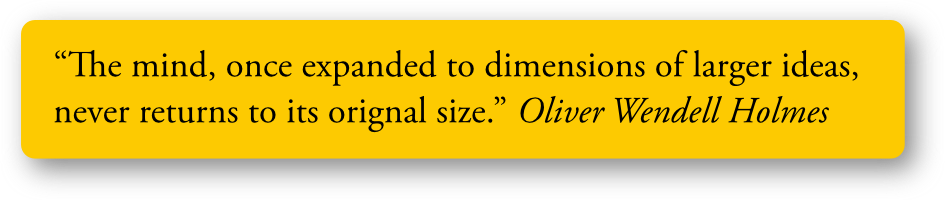
\includegraphics[width=12cm]{oliver}

    %“Insanity: doing the same thing over and over again and expecting different results.”
	%{\em Albert Einstein}

	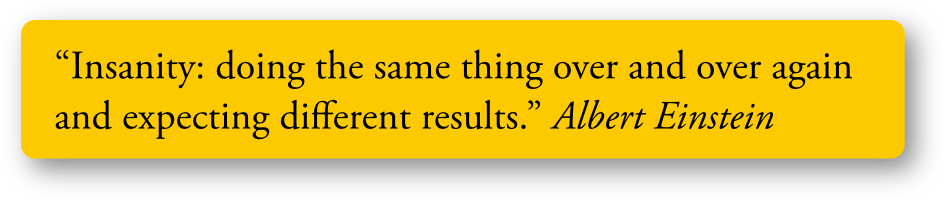
\includegraphics[width=12cm]{einstein}\label{img:einstein}

\end{minipage} \\
\end{flushright}

\vspace{1cm}

{\small Versão gerada em \\ \bf \today } % especifica a versão do PDF pelo dia que o gerou.
\end{center}
%\end{titlepage}
%%%%%%%%%%%%%   FIM DA CAPA E MINIPAGE %%%%%%%%%%%%%%%%%%%%%%%%%%%%%%%%%%%%%%%%%%

\tableofcontents

% ------------------------------------------------
%          FILE:  introducao.tex
%       CREATED:  Dom 30/Dez/2012 hs 15:57
%   LAST CHANGE:  2013 Apr 03 01:03:23 PM
%        AUTHOR:  Sérgio Luiz Araújo Silva
%          SITE:  http://vivaotux.blogspot.com
%       TWITTER:  @voyeg3r
%         SKYPE:  sergioaraujosilva
% -------------------------------------------------

\chapter{Introdução}\label{cha:intro}

% O comando \label{nome} define o marcador da parte especificada.
% Você pode citar esta seção usando o comando \ref{nome}.

Este livro contendo \pageref{LastPage} páginas é um convite ao auto
aprendizado, uma vez que ele cita dezenas de sites na Internet sendo um guia
para o seu trabalho individual de buscar conhecimento, colocamos aqui algumas
experiências com o intuito de lhe poupar esforço.  Compartilhe este material
com outras pessoas.

Ao longo deste livro você conhecerá uma série de técnicas
e dicas que tem como meta fazer com que você aprenda inglês
de forma mais rápida. Há mais de dois anos venho estudando
inglês e tenho conseguido excepcionais resultados. A soma
de toda essa experiência me levou a compartilhar as minhas
descobertas, tudo de bom que descobri estará aqui para
o deleite dos que tem o desejo sincero não apenas de
aprender Inglês, mas qualquer idioma.

\vspace{0.3\baselineskip}
\noindent
{\footnotesize \ding{42} Durante a leitura você verá vários trechos ou frases
em inglês, isso é proposital, você deverá copiar estas frases e
encontrar a tradução, isso é uma amostra de o quanto você vai
ganhar aprendendo mais inglês!}

\section{O primeiro passo}\label{sec:mil-palavras}

Dominar as palavras mais comuns de qualquer idioma é o principal fundamento,
pois com o domínio das mesmas você será capaz de rapidamente
abandonar o português e assistir vídeos com som e legendas totalmente em
inglês, obviamente que nosso objetivo final é que sejamos capazes de apenas
ouvir um falante nativo e poder entender 100\% do que foi falado.  O livro das
1000 palavras \index{Rubens Queiroz Almeida!1000 palavras} mais comuns da
lingua inglesa, de \index{Rubens Queiroz Almeida} {\em Rubens Queiroz
Almeida}\footnote{queiroz@iname.com}, foi criado à partir do
\index{Projeto Gutemberg} \href{http://www.gutenberg.org/}{{\em Projeto Gutemberg}}%
\footnote{http://www.gutenberg.org/} que digitalizou mais de
1600 livros que já estavam sob domínio público à época, este enorme acervo foi submetido
a um algoritmo\footnote{Programa de computador} que determinou quais são
as palavras mais comuns. Você pode baixar o livro das 1000 palavras mais
comuns do inglês neste link \href{http://goo.gl/jbyBZ}{http://goo.gl/jbyBZ} - Uma vez baixado o livro
você deverá ler as páginas introdutórias que explicam em detalhes
o objetivo do livro, em seguida você irá para o conteúdo propriamente
dito, à partir deste ponto você deve ler uma, duas ou mais páginas todo
dia, e assim você verá o seu vocabulário crescer em pouco tempo de forma
natural.

\vspace{0.3\baselineskip}
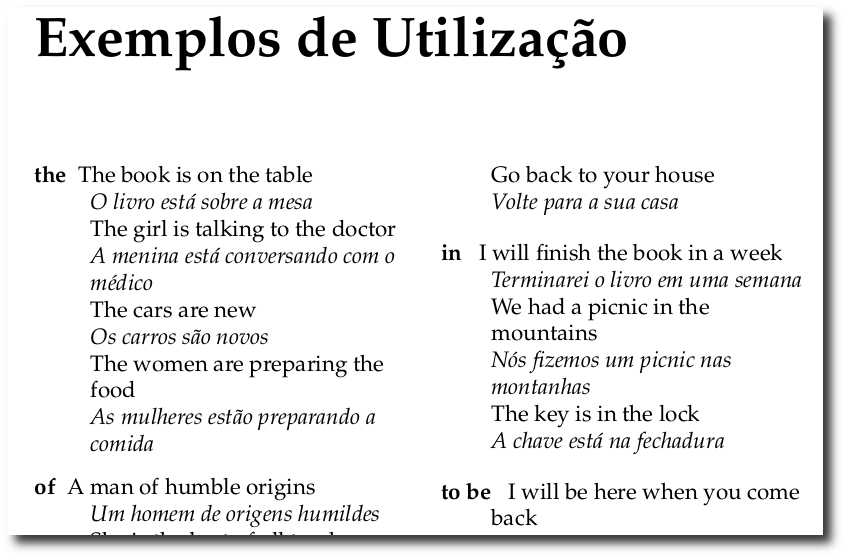
\includegraphics[width=0.8\textwidth]{1000-palavras}

\section{Técnicas Comprovadas por Pesquisas}

Citaremos ao longo do livro pesquisadores na área do ensino de idiomas que fizeram
descobertas que estão mudando a forma como as pessoas aprendem idiomas ao redor
do mundo.

\noindent
\vspace{0.8\baselineskip}
{\scriptsize \ding{42} ``Tell me and I forget, teach me and I may remember, involve me and I learn.'' -- Benjamin Franklin }

\subsection{Busque o nível adequado}

\noindent {\footnotesize \ding{42}
\href{https://blogdopedrojunior.wordpress.com/2010/05/08/estrategias-simples-para-expandir-o-seu-vocabulario-pt-1/}{Referência:
Aprenda inglês fácil.}}

\vspace{0.3\baselineskip} \noindent Você aprende muito mais rápido concentrando-se em
materiais que sejam de fácil entendimento. Esse é um dos pilares do método
desenvolvido pelo especialista em aprendizagem de idiomas, \index{Dr. Stephen
Krashen}
\href{http://adultesljobs.com/dr-stephen-krashen-on-language-acquisition/}{{\em
Dr Stephen
Krashen}}\footnote{http://adultesljobs.com/dr-stephen-krashen-on-language-acquisition/}.
Muitos acreditam que se aprende mais, estudando um material difícil de
entender.  De acordo com as pesquisas do {\em Dr. Krashen}, esse jeito não só
é menos eficiente, como também diminui a motivação do estudante.  Se
a quantidade de palavras não compreendidas for muito alta você ficará
naturalmente desestimulado, portanto busque materiais adequados ao seu nível. A única exceção é se você conseguir por exemplo livros bilingues, nos quais aparecem textos em duas línguas lado a lado, o que facilita a leitura. \\

\noindent
\vspace{0.3\baselineskip}
{\footnotesize \ding{42} Veja também a seção \ref{sec:estrategia} página~\pageref{sec:estrategia}.}

\noindent
{\footnotesize \ding{42} Leia também um artigo sobre o método do Dr.  Stephen Krashen neste
 \href{http://www.readability.com/articles/vdzq7x1o}{http://goo.gl/WCQIc}}

\subsection{Não estude gramática como foco principal}

Segundo estudos de pesquisadores como do \index{Dr. Marvin Brown}
\href{http://www.power-english.net/tag/j-marvin-brown}{{\em Dr. Marvin
Brown}}\footnote{http://www.power-english.net/tag/j-marvin-brown} que
desenvolveu o método \index{Dr. Marvin Brown!Listening Approach} ``The
Listening Approach'', o estudo da gramática na verdade atrapalha o aprendizado,
lembre-se que as crianças quando aprendem a falar apenas ouvem por dois anos ou
mais.  A menos que você seja professor de português eu diria que você não
lembra sequer 1/4 das regras gramaticais que você aprendeu na
escola, no entanto você consegue se expressar bem e também perceber quando
alguém comete um erro de português!

\subsection{Motivos para não estudar gramática}\label{sub:not-grammar}
\index{Gramática}

Você não necessita conhecer os detalhes técnicos de um idioma para usa-lo,
do memo modo que não precisa entender o funcionamento interno de um motor para dirigir
um carro, ou ainda não necessita saber como um processador de computador funciona
para navegar na internet.

Crianças de 4 anos falam sua lingua materna sem saber um vírgula sequer sobre
gramática, se seus pais falam errado elas também falam errado, se seus pais
falam corretamente elas também falam corretamente. Juntando o que aprendemos
sobre o fato de as crianças aprenderem a falar um idioma apenas pelo convívio
podemos somar a isso a ação consciente de anotar sempre as frases inteiras, nas
quais estarão implícitas todas as regras gramaticais. Há ainda outra vantagem
em anotar as frases inteiras, com o tempo você perceberá que sua capacidade de
inferir\footnote{Deduzir o sentido das palavras pelo contexto} o sentido
das palavras pelo contexto irá melhorar substancialmente.

\vspace{0.3\baselineskip}
\noindent
{\footnotesize \ding{42}  Veja como estudar inglês de forma indireta na seção~\ref{sec:EnglishLife}
página~\pageref{sec:EnglishLife}}

\vspace{0.3\baselineskip}
\noindent
{\footnotesize \ding{42}  ``Don't say people you are learning English, just
talk to them about a topic you are interested in \dots ``}

% colocar o link sobre o listening approach
\subsection{Aprenda contextualmente}\label{sub:aprenda-contextualmente}
\index{Aprenda contextualmente}

Quando você se deparar com uma nova palavra não anote apenas a palavra, anote
a frase em que ela se encontra, assim você estará aprendendo a gramática pelo
contexto, ou seja, seu cérebro vai aprender a gramática sem que isso seja uma
preocupação explícita, portanto siga essas duas dicas:

\begin{itemize}
     \item{Não anote palavras isoladas}
     \item{Não estude gramática}
\end{itemize}

\noindent
Entre as muitas vantagens de se estudar frases inteiras citamos o aprendizado
de vocabulário comum a situações específicas veja o exemplo:

\begin{figure}[h!]
	\centering
	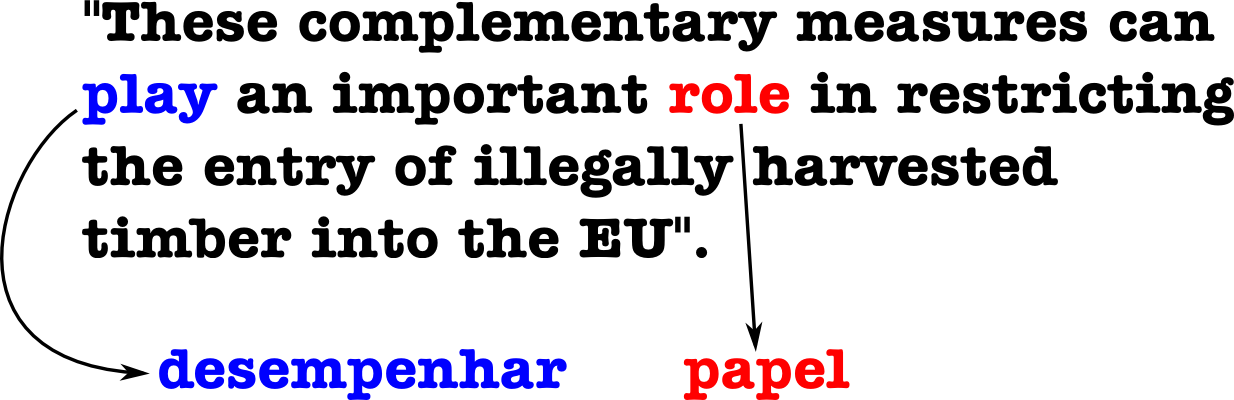
\includegraphics[width=0.8\textwidth]{play-role}
	\caption{play-role}
\end{figure}

\index{Aprenda contextualmente!Linguee} Uma forma interessante de aprender
novas palavras dentro do contexto é através do site linguee
\href{http://www.linguee.pt/}{http://www.linguee.pt/}, nele você escolhe
o idioma de entrada e o de saída e recebe vários textos de exemplo com
a palavra buscada.

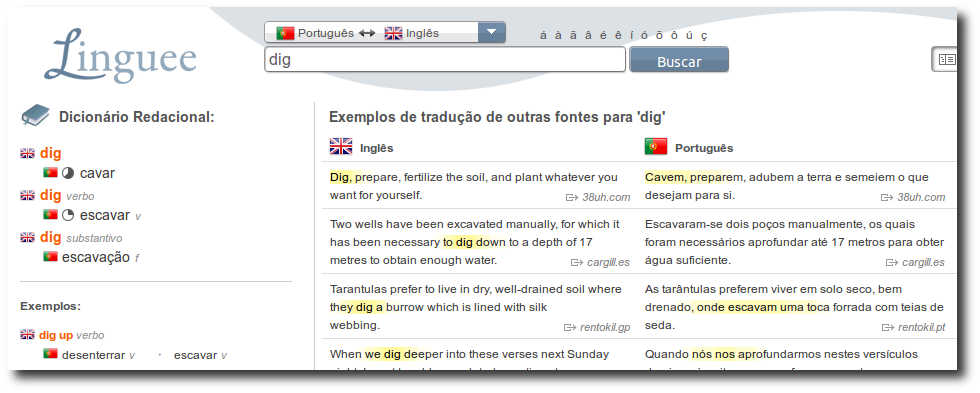
\includegraphics[width=\textwidth]{linguee-exemplos}

\noindent
{\footnotesize \ding{42} Um bom dicionário com exemplos pode ser acessado neste link \href{http://www.yourdictionary.com/}{http://www.yourdictionary.com/} }

\noindent
Outro site muito bom para expandir o vocabulário de {\bf estudantes avançados} é o site
\href{http://www.vocabulary.com}{http://www.vocabulary.com}, com muitos desafios.
\index{Vocabulario}

\begin{figure}[h!]
	\centering
	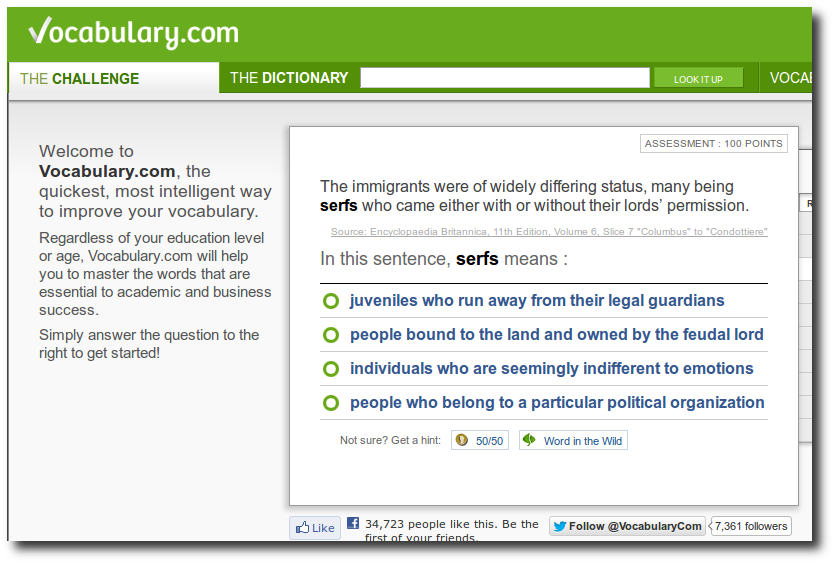
\includegraphics[width=0.8\textwidth]{vocabulary-one}
\end{figure}

% \begin{figure}[h!]
% 	\centering
% 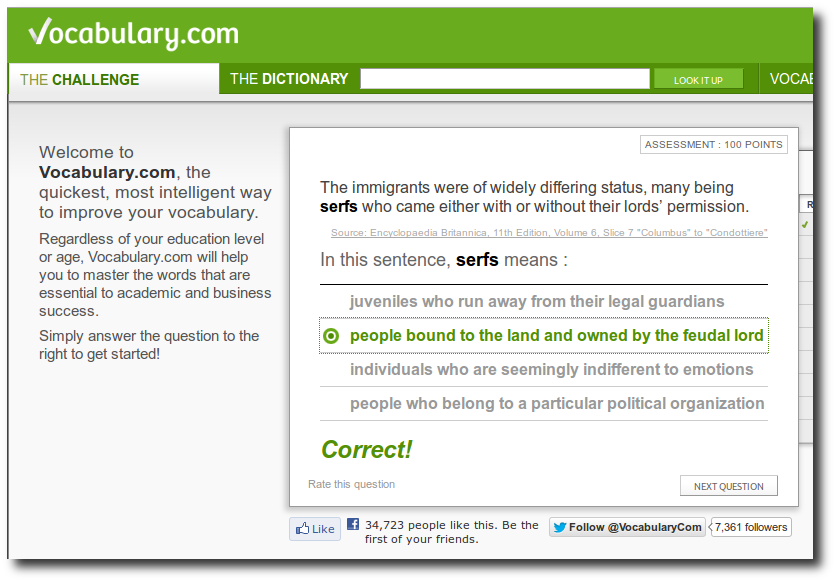
\includegraphics[width=12cm]{vocabulary-two}
% \end{figure}

\noindent
\vspace{0.3\baselineskip}
{\footnotesize \ding{42}  ``English {\em students} learn to pronounce words {\em individually},
and that's why they don't understand native speakers in conversations.''}

\vspace{0.3\baselineskip}
\noindent
{\footnotesize \ding{42} Veja como ter uma espécie de livro de anotações online
na seção~\ref{sec:evernote} página~\pageref{sec:evernote}}

\subsubsection{Leia textos bilíngues}
\label{ssub:leia_textos_bil_ngues}

\begin{multicols}{2}

\noindent
If you work daily with bilingual texts your capacity of understand the
meaning of phrases will rise alarmingly. This exercise will be so
natural to your brain that one day you will notice yourself reading
complicated texts withou any effort.

\noindent
This sort of activity puts you
in a kind of imersion and at same time gives you real context in wich
you will have access rapidly to the translated version, all this make
you acquire the needed skills you must absorb to improve your level faster.

\columnbreak

\noindent
Se você trabalha diariamente com textos bilíngües sua capacidade de
compreender o significado de frases vão subir de forma alarmante. Este
exercício será tão natural para o seu cérebro que um dia você vai
notar-se ler textos complicados withou qualquer esforço.

\vspace{0.5cm}
\noindent
Esse tipo de atividade coloca em uma espécie de imersão e ao mesmo tempo dá-lhe
contexto real no qual você terá acesso rápido para a versão traduzida,
tudo isso faz você adquirir as habilidades necessárias que você
precisa absorver para melhorar o seu nível mais rápido.

\end{multicols}

\pagebreak

\begin{multicols}{2}

During the elaboration this book, more precisely these two columns I
was writing directly the text in Google Translator and copying the
result to this section. In this moments my brain was accessing my
memories to convey you all ideas I needed to you understand this idea.

\vfill \columnbreak

Durante a elaboração deste livro, mais precisamente essas duas colunas eu estava escrevendo
diretamente o texto no Google Tradutor e copiar o resultado para esta
seção. Neste momento o meu cérebro estava acessando minhas memórias
para transmitir-lhe todas as idéias que eu precisava para você
entender esta idéia.

\end{multicols}

% subsubsection leia_textos_bil_ngues (end)


\subsection{Fale sem pensar, fale automaticamente}

Se você estudar muito gramática, toda vez que for falar você tenderá
a traduzir, pensar de forma consciente sobre a gramática, encontrar uma
resposta, traduzir novamente para o inglês, instante no qual a conversa ficará
truncada e anti-natural. Obviamente se você nunca conseguir fazer a sua
conversação fluir um pouquinho que seja, sua confiança também vai pro espaço.

\subsubsection{Lições de conversação}
\label{ssub:li_es_de_conversa_o}

Na verdade a gramática é importante, mas ela não o ajudará a entender
a conversação do dia-a-dia ou a falar inglês naturalmente e
fluentemente sem se sentir embarassado. O único caminho para tornar-se
um falante efetivo em inglês é praticando ouvir e falar tanto quanto
possível. Este trecho foi retirado do site
\href{http://www.englishwithjo.com/english-conversation-lessons/}{http://www.englishwithjo.com/english-conversation-lessons/}
e essas considerações fazem muito sentido, não acha?

Para criar esse tipo de interação você pode criar \emph{Flashcards}
(veja mais sobre os Flashcards na seção~\ref{sub:programas_para_memoria_o} página\pageref{sub:programas_para_memoria_o}) contendo perguntas
cotidianas, de um lado a pergunta em inglês, do outro a resposta. Com
o tempo você vai reformulando os cartões para criar respostas mais
elaboradas. Lembre-se de ler as perguntas e respostas em voz alta para
praticar o listening e a pronúncia.

{\footnotesize \ding{42} Ao ler em voz alta ativamos o lóbulo frontal
do cérebro, que entre outras coisas é responsável pela linguágem.}

% subsubsection li_es_de_conversa_o (end)


\subsection{Repetição}

O nosso cérebro necessita de muitas repetições para gravar novos conhecimentos,
portanto não tenha tanta ânsia por novas lições, uma lição simples mas
explorada de várias formas tais como, fazendo a tradução do texto para
o português, gravando sua voz à partir do conteúdo do texto, a audição do mesmo
material, a transcrição do audio etc.  farão com que seu cérebro assimile mais
rapidamente o conteúdo. A ideia é esgotar todas as possibilidade de aprendizado
em cada lição. Certa vez foi perguntado ao \index{Michael Jordan} {\em Michael
Jordan}\footnote{Talvez o maior jogador de basquete da história} como ele se
tornara um jogador fora do comum, ele respondeu dizendo: ``fundamento,
fundamento, fundamento'', ou seja, ele disse que considerava o estudo dos
fundamentos como sendo o mais importante para se tornar um bom jogador.

Outro aspecto a ser considerado é com relação ao intervalo das
repetições, 10 repetições de 1 minuto em intervalos regulares é mais
eficaz que duas horas ininterruptas de estudo, pois o cérebro vai
cansando e pelo fato de não haver futuras repetições o cérebro tenderá
a descartar essa informação. \emph{Veja mais adiante no texto sobre a
curva de esquecimento}.

Veja como determinação e uso da repetição são bases fundamentais para
o aprimoramento e excelência: \index{Airton Senna} {\em Airton Senna da Silva}
um dos maiores pilotos de Fórmula
1 da história certa vez perdeu uma corrida por causa da chuva, ele disse que
jamais perderia uma corrida por esse motivo, e como ele morava em frente ao
autódromo de Interlagos, toda vez que começava uma chuva, ele vestia
o macacão, entrava no carro e ia correr na chuva, moral da história, ele se
tornou um ``expert'' em corridas de chuva. Claro que houve na história
pessoas que nasceram com talento natural para certas atividades, contudo
o esforço, o treinamento potencializa sobremaneira suas possibilidades.

\subsection{A curva de esquecimento}
\label{sub:a_curva_de_esquecimento}
Referência: \href{http://goo.gl/7kbTo}{http://goo.gl/7kbTo}

\begin{figure}[h!]
	\centering
	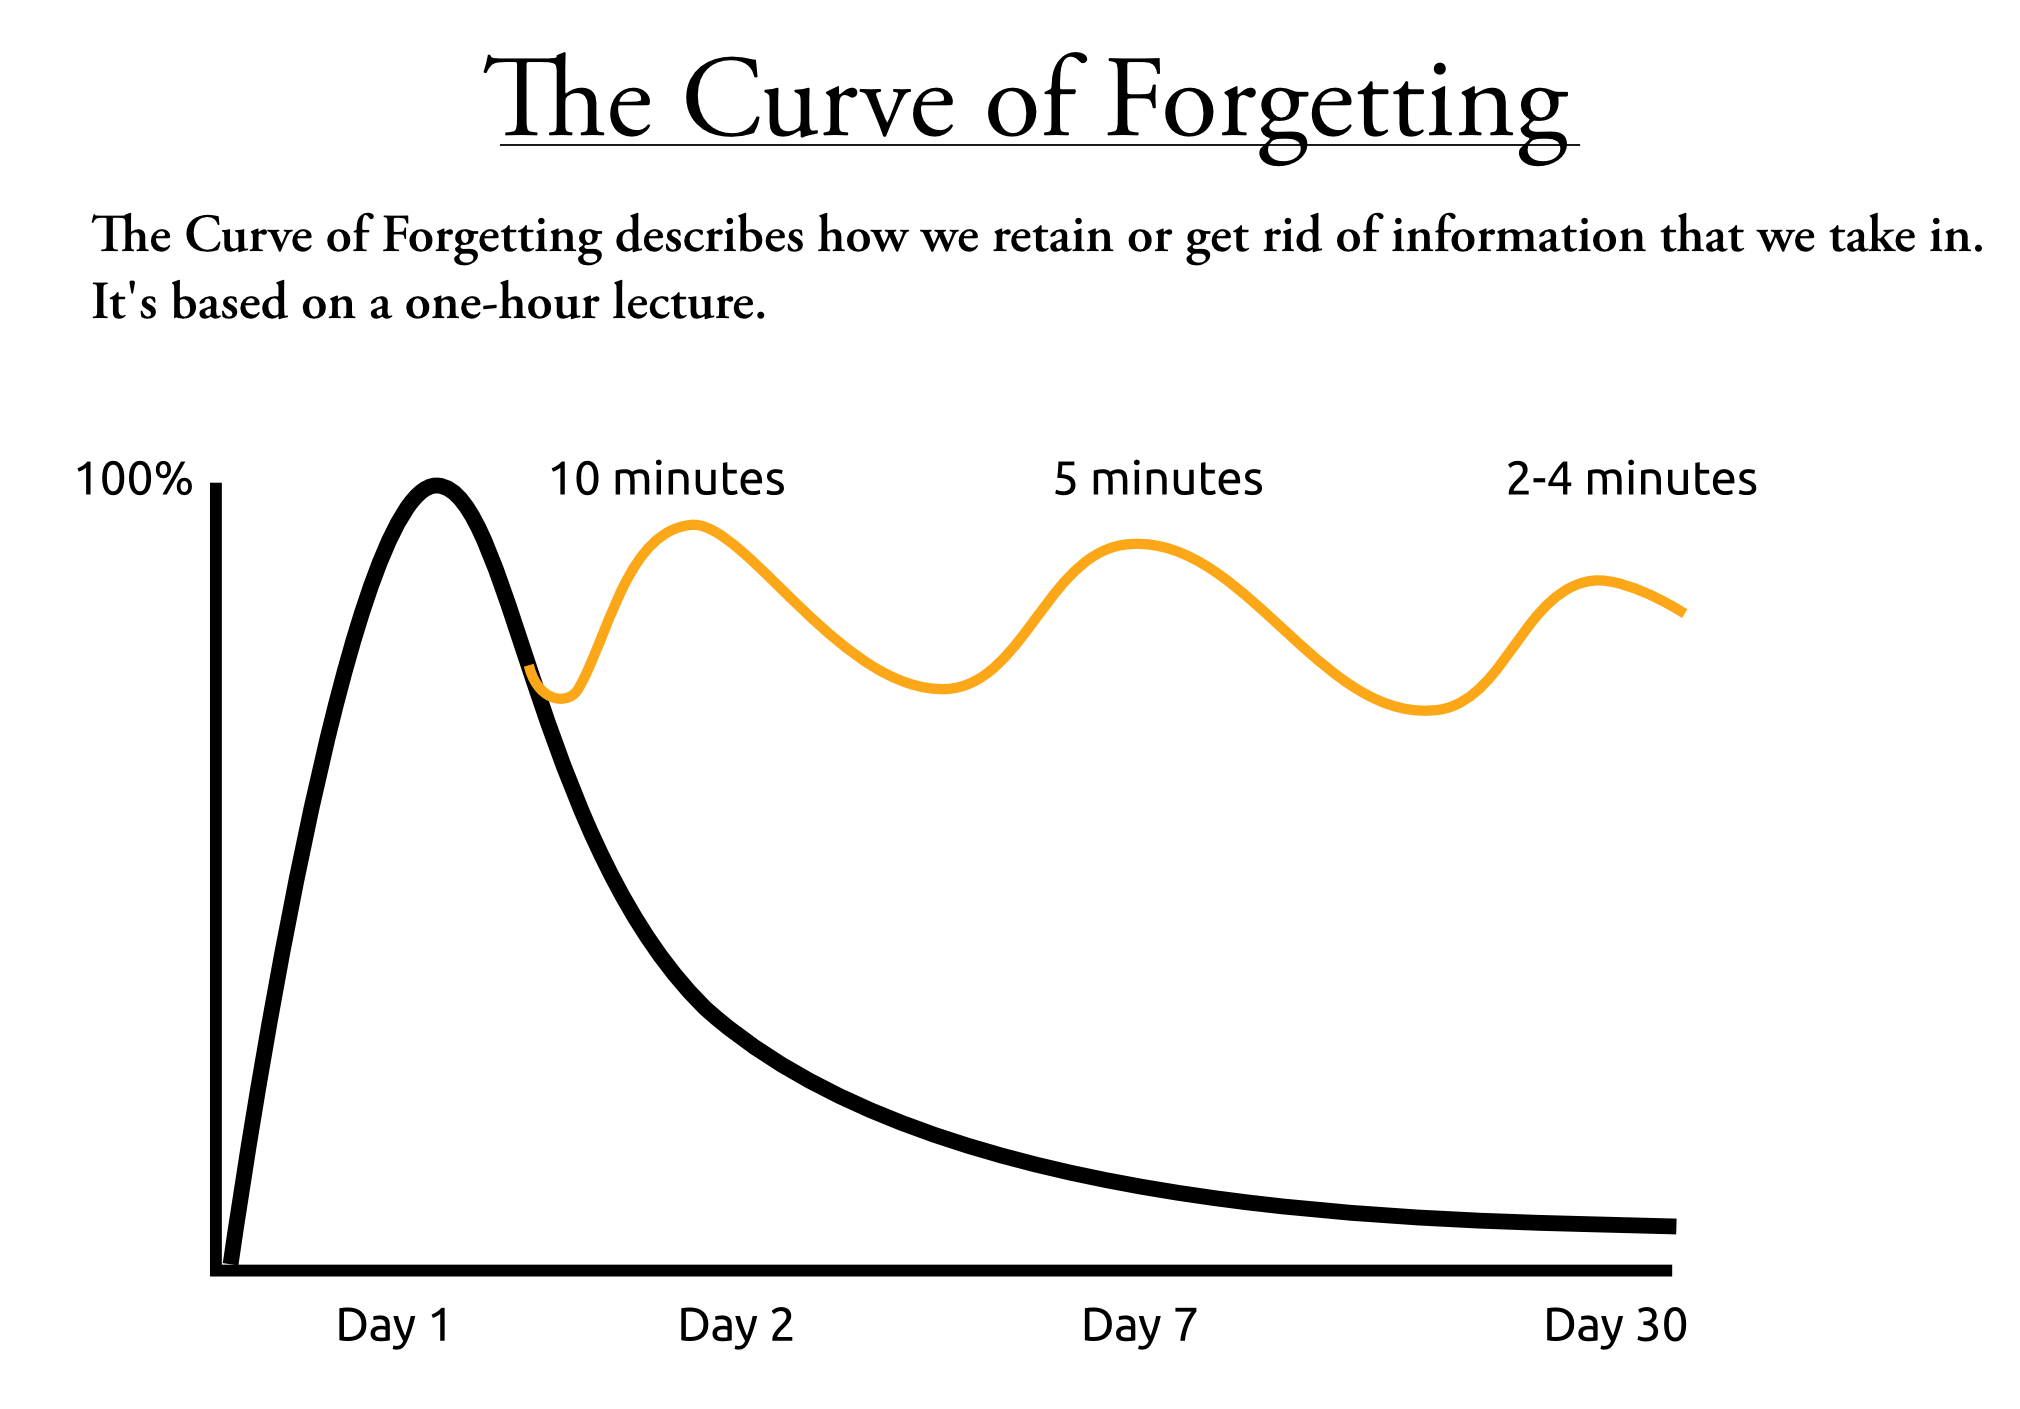
\includegraphics[width=0.8\textwidth]{forgeting-curve}
	\caption{forgeting-curve}
\end{figure}

No 1º dia, no início do estudo, você vai do ponto onde não sabe nada, ou 0\%, (onde a
curva começa na linha de base). No final do estudo você sabe 100\% do
que você estudou, onde a curva sobe para seu ponto mais alto.

No 2º dia, se você não fez nada com a informação que você aprendeu na
aula, não pensou sobre isso novamente, leu de novo, etc, você terá
perdido 50\% -80\% do que você aprendeu. Nossos cérebros estão
constantemente gravando informações em uma base temporária: pedaços de
conversas ouvidas na calçada, o que a pessoa na frente de você está
vestindo. Porque a informação não é necessária, e não vem de novo,
nossos cérebros descartam tudo isso, juntamente com o que foi aprendido
na estudo que você realmente deseja memorizar!

No 7 º dia, lembramos ainda menos, e no dia 30, mantemos cerca de 2\%
-3\% da hora original! Este bem coincide com os exames de meio do
bimestre, e pode ser responsável por nos fazer sentir como se nunca
tivéssemos visto aquilo antes.


É possível alterar a forma da curva! Reprocessando o mesmo bloco de
informações, enviando assim um grande sinal para o cérebro para
segurar esses dados. Quando a coisa se repete, seu cérebro diz: "Oh -
lá está ele de novo, é melhor eu manter isso." Quando você está
exposto à mesma informação várias vezes, leva-se menos e menos tempo
para "ativar" a informação em sua memória de longo prazo, e torna-se
mais fácil para você recuperar as informações quando você precisar
delas.

Aqui está a fórmula e o motivo para arrumar tempo de rever seu
material de estudo: Dentro de 24h da absorção da informação gaste 10
minutos revendo e você subirá a curva de memorização para quase 100\%
novamente. Uma semana depois (sete dias), levará apenas 5 minutos para
``reativar'' a mesma informação, e novamente elevar a curva. Em 30 dias,
seu cérebro necessitará de algo entre 2 e 4 minutos para lhe retornar
resultados, ``Sim, Eu sei disso\dots''

Frequentemente os estudantes acham que não conseguirão achar tempo para uma
revisão diária em sua agenda - Eles encontram problemas em manter o
rítmo. Noentanto, esta revisão é um excelente investimento de tempo.
Se você não revisar, você necessitará de 40 a 50 minutos reaprendendo
cada hora de material mais tarde - você tem tanto tempo assim?

Estudar exastivamente raramente proporcionará a retenção de
informações na memória de longo prazo de maneira satisfatória,
tornando difícil a recuperação dessas informações quando form
necessárias.

Dependendo do ritmo do seu estudo, a recomendação geral é gastar
meia hora no final de cada dia, e 1.5 a 2 horas cada final de semana
em atividades de revisão. Talvez você tenha tempo apenas para revisar
4 ou 5 dias da semana, e a curva se mantem na metade. Ok, é bem melhor
do que 2 a 3\% de retenção se você não fizer revisão alguma.

Muitos estudantes ficam maravilhados com a diferença proporcionada pelas
revisões regulares e em o quanto bem eles entendem e reteem materiais.
Vale a pena experimentar por algumas semanas, apenas pra ver a diferença
que isso fará para você!.

% subsection a_curva_de_esquecimento (end)

\subsection{Programas para memorização}
\label{sub:programas_para_memoria_o}

\noindent
Um excelente programa para trabalhar a memorização dentro dos intervalos
ideais de revisão chama-se \emph{Anki} o mesmo pode ser baixado para
Windows, Linux, Mac ou Android neste link \href{http://ankisrs.net/}{http://ankisrs.net/},
sua utilização é simples contudo segue também um link de um vídeo
sobre sua utilização básica \href{http://goo.gl/ueyFv}{http://goo.gl/ueyFv}

\vspace{0.3cm} \noindent {\footnotesize \ding{42} Leia um exceptional
artigo sobre o anki
\href{http://www.davidmansaray.com/anki-srs}{http://www.davidmansaray.com/anki-srs}
} \vspace{0.5\baselineskip}

\noindent
{\footnotesize \ding{42} If you are not willing to learn, no one can help you. If you are
determined to learn, no one can stop you. }
\vspace{0.3\baselineskip}

\noindent
Existe uma técnica de memorização chamada \href{http://goo.gl/Y5pRj}{repetição espaçada}
que consiste em repetir um pequeno trecho em intervalos regulares ao invés de
concentrar-se em uma seção longa de estudo, segundo estudos este
método é mais efetivo para memorização. De fato faz muito sentido, já
que quando estudamos por um longo período sem descanso nosso poder
de concentração diminuir. Outro fator é que o cérebro funciona de tal
forma que quando algo e visto mais de uma vez ele tende a reter, como
se ele ``pensasse assim'': Eu já vi isso uma vez, é melhor eu guardar
essa informação, neste caso ele guarda na nossa memória de longo prazo.

\vspace{0.3\baselineskip}
\noindent
Você pode recortar uma cartolina formando os cartões e preenche-los
de um lado com uma frase em inglês e do outro com sua tradução,
utilize cores para tornar os cartões mais atraentes.


\newpage
\begin{figure}[h!]
	\centering
	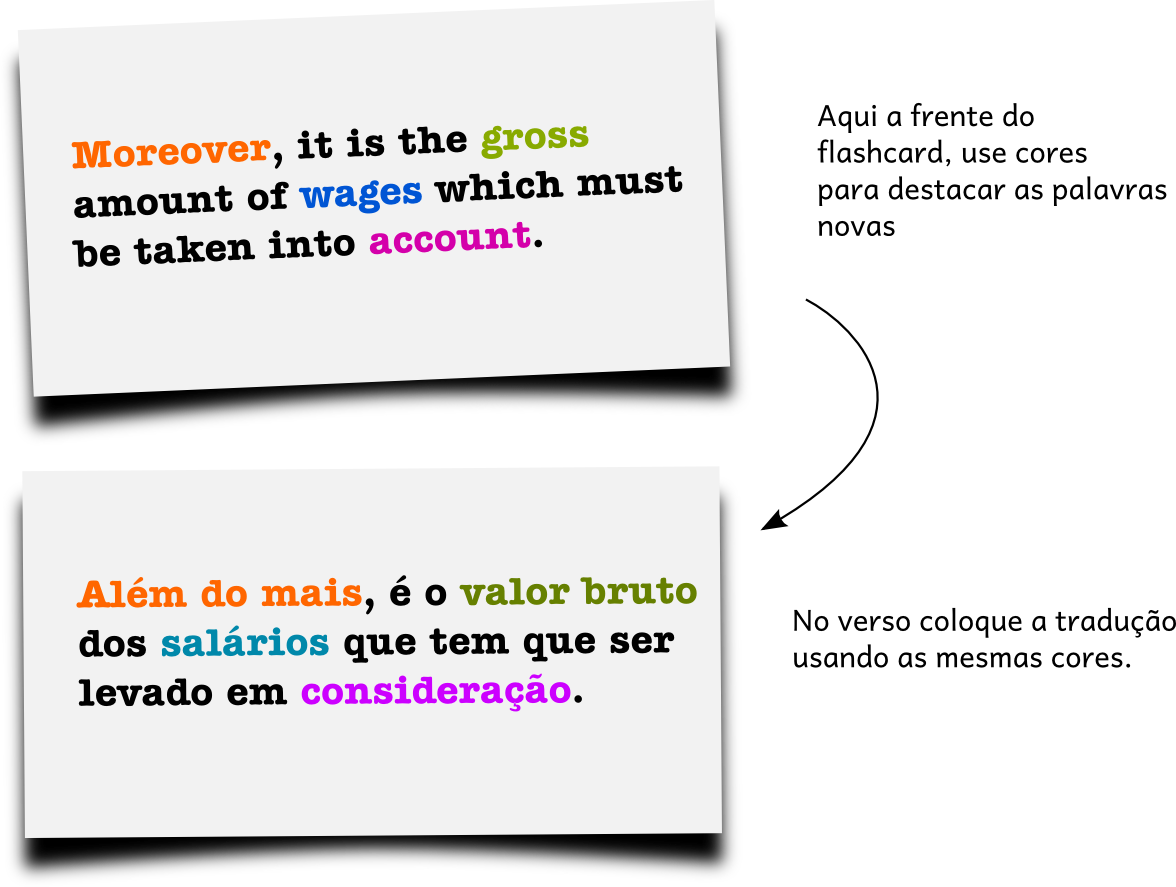
\includegraphics[width=0.8\textwidth]{flashcard}
	\caption{flashcard}
\end{figure}

% subsection programas_para_memoria_o (end)


\subsection{A pirâmide do aprendizado}
\label{sub:a_pir_mide_do_aprendizado}

Outro aspecto a ser considerado acerca da memoriação é quão eficientes
somos em gravar a informação inicial, ou seja, não adiantam muitas
técnicas de momorização para o que não foi sequer absorvido, é aí que
entra a \emph{Pirâmide do aprendizado}, que nos mostra através de pesquisas
feitas pela Universidade de Queens em Belfast, dados sobre quais são
os métodos de estudo mais eficientes para reter a informação inicial.
Ou seja, quais métodos geram uma melhor impressão em nossos cérebros.

\begin{figure}[ht!]
	\centering
	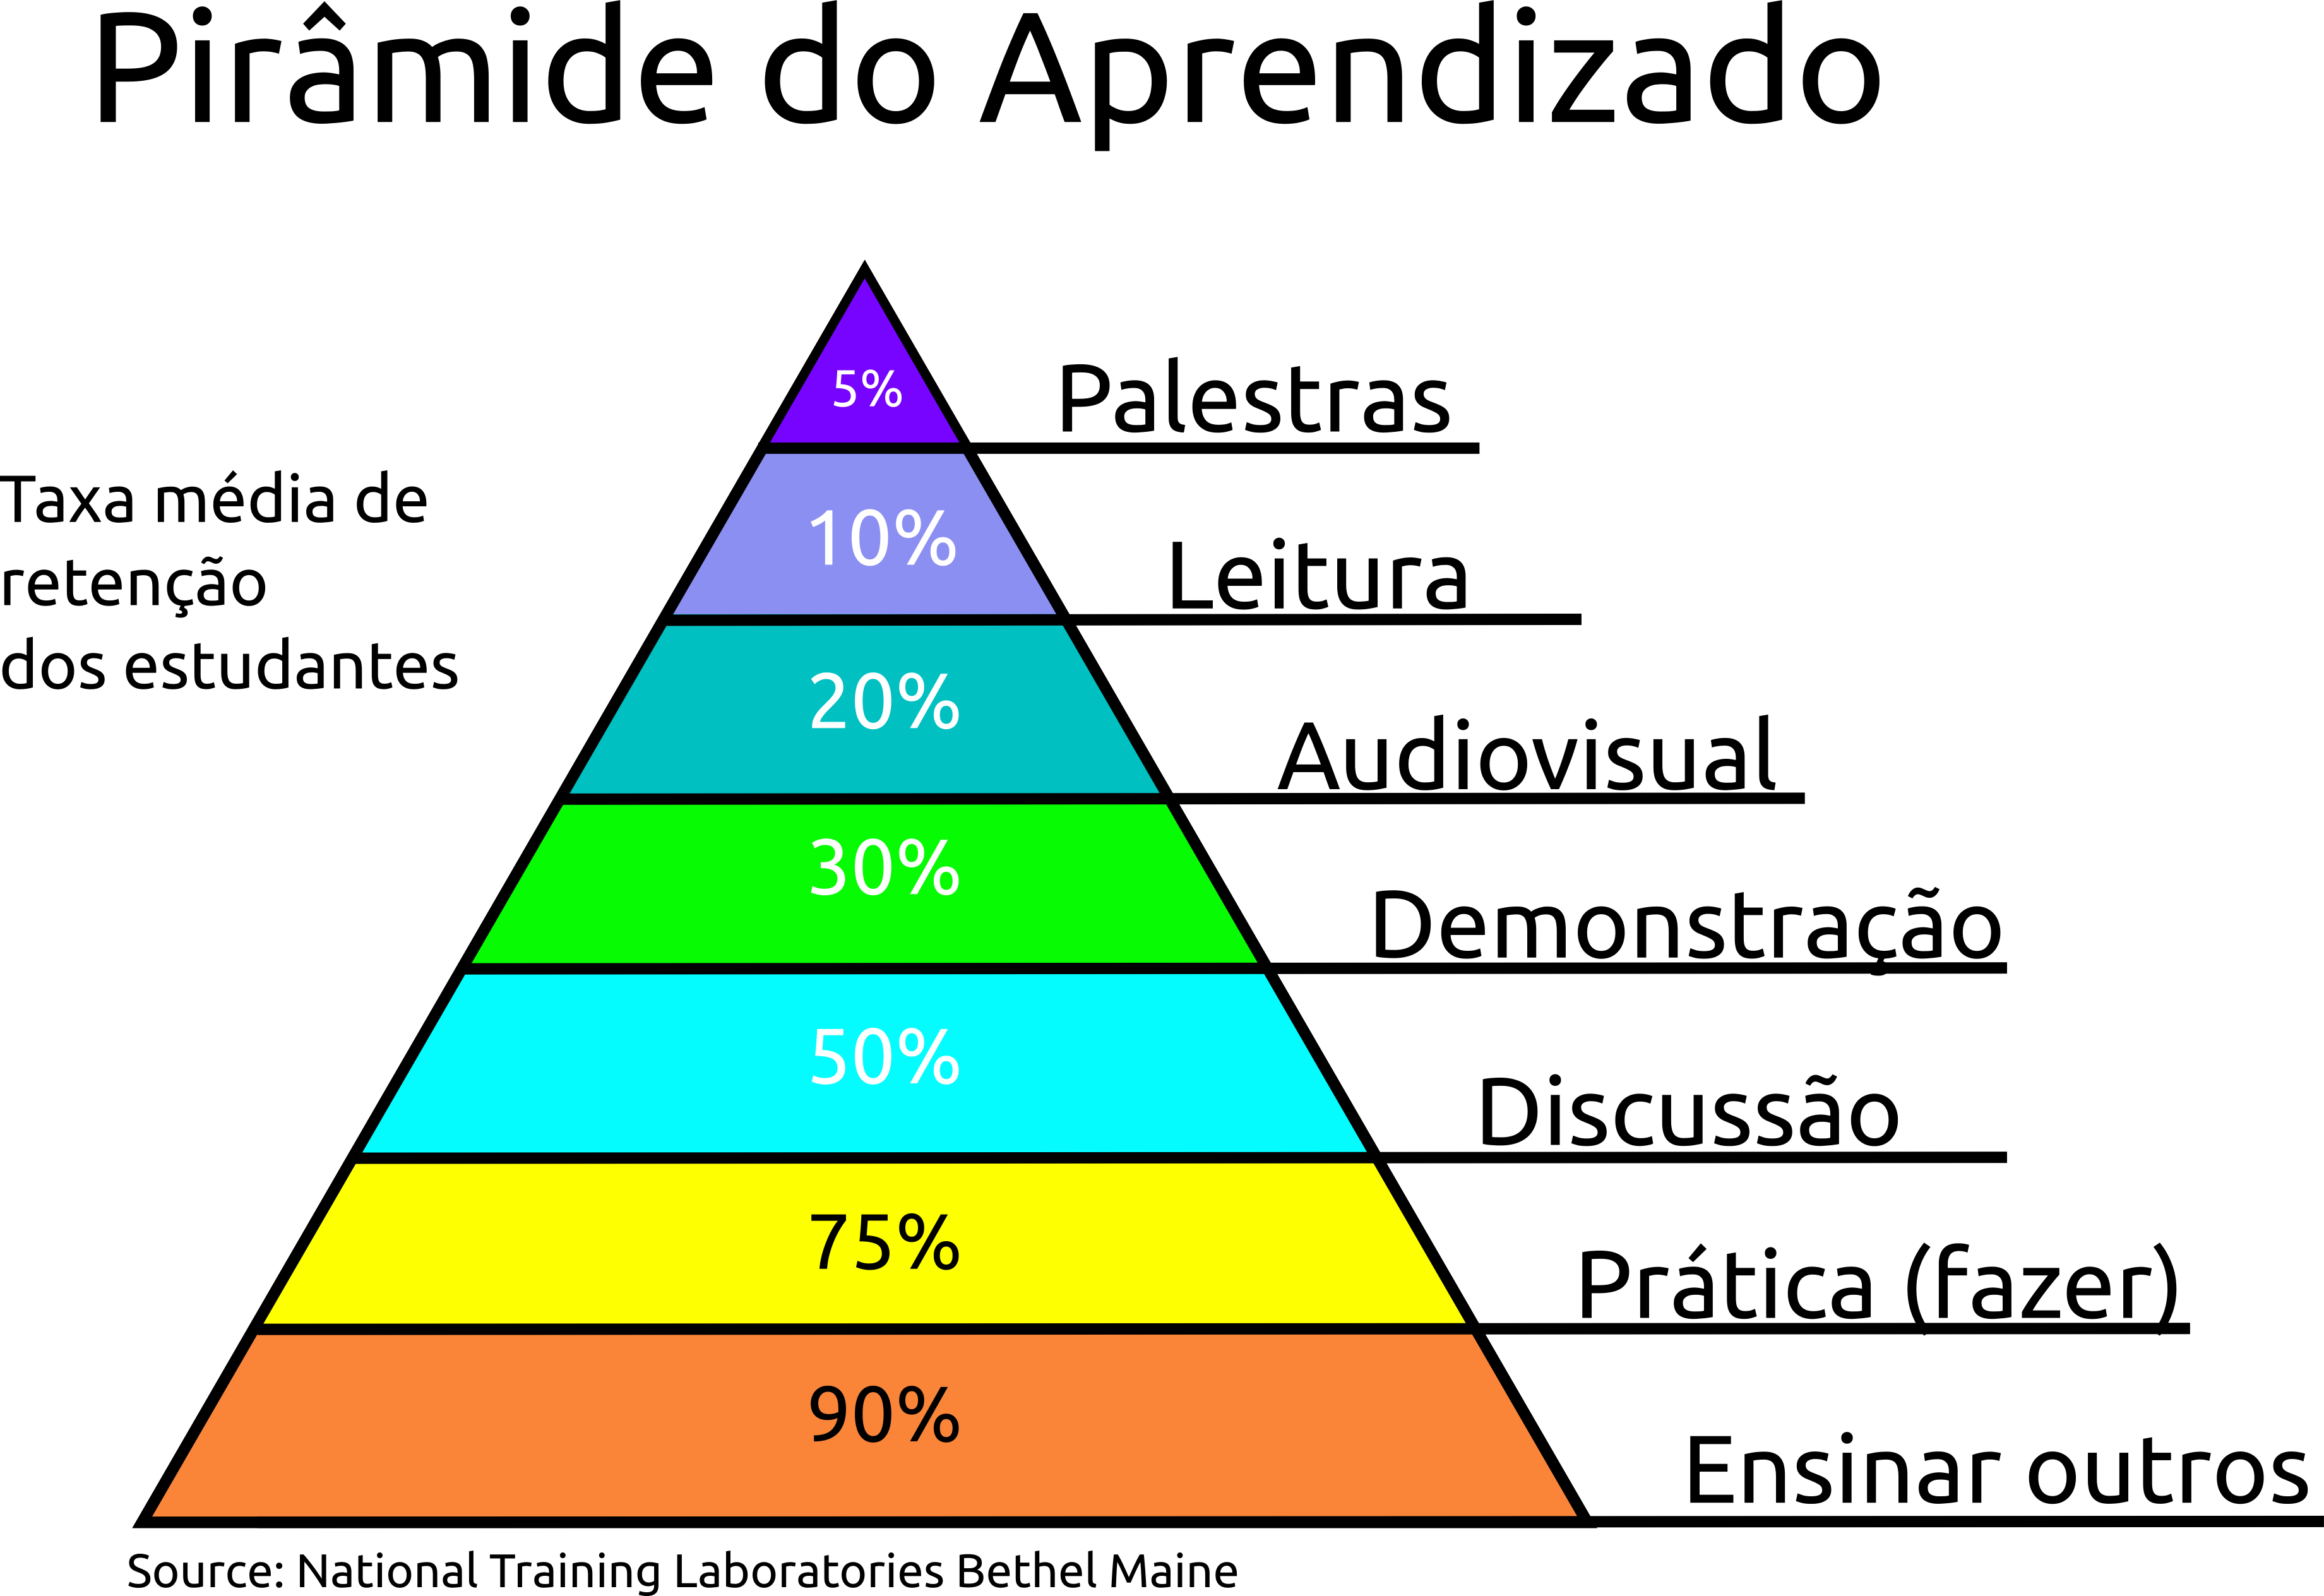
\includegraphics[width=0.6\textwidth]{piramide-do-aprendizado}
	\caption{piramide-do-aprendido}
\end{figure}

\newpage
O modelo proposto pela \emph{Pirâmide do aprendizado} está sendo
questionado por muita gente na internet basicamente com a seguinte
argumentação, se uma palestra for feita por alguém bem preparado
gerará mais retenção de aprendizado do que o ato de ensinar feito
por alguém menos preparado, ou coisa do tipo, mas na verdade a
proposta da pirâmide se resume a:

\begin{description}
	\item [ação] Os estudantes devem ser expostos a métodos de aprendizado ativos, isto significa que uma
		palestra que em geral tem baixo nível de retenção, caso envolva
		emocionalmente a plateia, caso crie interações com a mesma, elevará o
		seu nível de retenção. Isso explica o fato de que boas
		palestras geram mais retenção.
	\item [solução de problemas] O conhecimento deve ser absorvido através de compartilhamento e solução de problemas
	\item [pensar] Os estudantes devem, analizar sintetizar e avaliar
\end{description}

% subsection a_pir_mide_do_aprendizado (end)

\subsection{Aprendizado consciente e acidental}
\label{sub:aprendizado_consciente_e_acidental}

Durante sua jornada de aprendizado procure equilibrar a quantidade
de tempo dedicado ao estudo consciente e ao estudo casual, a diferença
entre ambos é descrita abaixo de forma simples.

\begin{description}

	\item[Aprendizado deliberado ou consciente] Acontece quando você
		etuda inglês, talvez você sublinhe palavras que você não
		conhece em um jornal, artigo ou em um livro, então abre o
		dicionário, cria flashcards (leia sobre o anki na
		página~\pageref{sub:programas_para_memoria_o}), estude
		gramática etc. Você ativamente tenta aprender e lembrar
		inglês.

	\item[Aprendizado acidental] Acontece quando você não está
		tentando aprender, ou memorizar nada - você está apenas se
		divertindo. Por exemplo: enquando você ouve um podcast, lê um
		livro e ... uma palavra ou frase salta em sua frente. Talvez
		você venha tentando lembrar aquela palavra antes e não
		conseguiu memoriza-la ainda, mas desta vez o contexto ajuda
		você de tal forma que vem aquele estalo na mente "Ah-Há!".
		Neste momento você não mais irá esquecer aquela palavra, isto
		é o aprendizado acidental.

\end{description}

Quando você deliberadamente tenta aprender uma palavra você a coloca
em sua memória, quando você escuta uma palavra acidentalmente você cria
um link entre a palavra na memória e a mesma palavra no contexto e a
fixa em seu cérebro.

Tente criar a maior número de oportunidades para o aprendizado
acidental possível, seja colocando filmes com som inglês e legenda em
português e vice-versa, seja ouvindo podcasts na fila do banco etc. No
futuro, quando você tiver um bom vocabulário, uma boa forma de unir o
aprendizado acidental com o consciente é estudar inglês ouvindo um
falante nativo do inglês lhe ensinando inglês, mas lembre-se que para
isso você deve ler o livro das \emph{1000 palavras mais comuns do
ingês}\footnote{http://goo.gl/jbyBZ} citado anteriormente, em minha
experiência pessoal este livro foi fundamental e o será também para
você!

\vspace{0.3\baselineskip}
\noindent
{\footnotesize \ding{42} Muitas pessoas acabam focando por demais em um dos dois métodos,
sendo que o ideal o balanceamento entre os dois, tanto deliberado como
casual}.


% subsection aprendizado_consciente_e_acidental (end)

\newpage
\subsection{Interação}\label{sub:interacao}

O professor americano \index{H.J Hoge} ``H.G Hoge'' criou o método \index{H.J
Hoge!Effortless English}
\href{http://www.effortlessenglishpage.com/p/7-rules.html}{``Effortless
English''}\footnote{Inglês sem esforço:
http://www.effortlessenglishpage.com/p/7-rules.html} ou  Inglês sem Esforço
-- para saber mais acesse este endereço:
\href{http://goo.gl/DyfZ7}{http://goo.gl/DyfZ7} -- basicamente este método usa
mini-histórias com as quais o ouvinte tem que interagir, a história é contada
e em seguida, frase por frase, são feitas várias perguntas na qual você deve
dar respostas. O conteúdo da história é bem simples para que as respostas seja
automáticas o usuário deve repetir a audição da mini história durante uma ou
duas semanas a fim de conseguir o que o professor ``HG Hoge'' chama de ``Deep
Learning'' ou aprendizado profundo no qual o estudante não tem sequer que pensar
nas respostas, as mesmas surgem naturalmente, o método é fortemente baseado na
repetição. Aqui um link
\href{http://goo.gl/ECXTr}{http://goo.gl/ECXTr}
do torrent\footnote{Protocolo de rede para permitir downloads mais rápidos}
para o curso, em que você terá que baixar um arquivo tar.bz2, descompactar e só
então terá o torrent. {\footnotesize \ding{42} É possível que ele exiba uma
janela ``pop-up.''}

Na verdade, o sistema {\em Effortless English} foi projetado com base em várias
pesquisas feitas pelos maiores especialistas e doutores em aprendizagem de idiomas no
mundo: Stephen Krashen, James Asher, J. Marvin Brown, Ashley Hastings, Brenda Murphy, David Long e Blaine Ray.

\vspace{0.3\baselineskip} \noindent {\footnotesize \ding{42}
``\dots Formular regras e ensinar fatores complexos sobre a lingua alvo
não é ensino de línguas, mas ao contrário é `apreciação da língua' ou linguística.''
\href{http://www.readability.com/articles/ndsyiy1q}{{\em Stephen Krashen}}}

\vspace{0.3\baselineskip} \noindent {\footnotesize \ding{42} ``Acquisition requires
meaningful interaction in the target language - natural communication - in
which speakers are concerned not with the form of their utterances but with
the messages they are conveying and understanding.''
\href{http://www.readability.com/articles/ndsyiy1q}{{\em Stephen Krashen}}}

\vspace{0.3\baselineskip} \noindent {\footnotesize \ding{42} ``In the real world,
conversations with sympathetic native speakers who are willing to help the
acquirer understand are very helpful.''
\href{http://www.readability.com/articles/ndsyiy1q}{{\em Stephen Krashen}}}

\begin{figure}[h!]
	\centering
	\caption{Dr Stephen Krashen em uma palestra}
	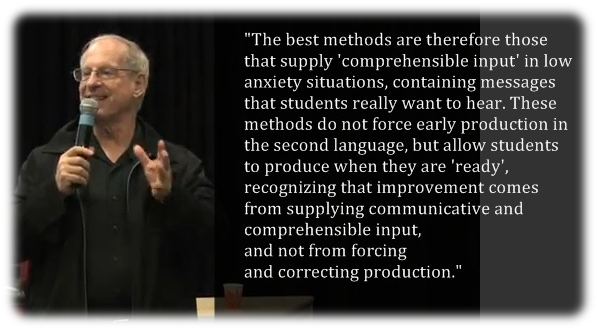
\includegraphics[width=0.8\textwidth]{input}
\end{figure}

\vspace{0.3\baselineskip}
\noindent
``Os melhores métodos são portanto os que fornecem `entrada compreensível'
em situações de baixa ansiedade, contendo mensagens que os estudantes realmente
querem ouvir. Estes métodos não forçam a produção precoce em uma segunda linguagem, mas
permitem aos estudantes produzir quando eles estiverem prontos, reconhecendo
que a melhora vem pelo suprimento de mensagens inteligíveis, e não forçando e
corrigindo o que foi produzido.'' {\em Stephen Krashen}


\newpage
%\vspace{-1.2cm}
\section{Como usar o google para aprender inglês}\label{sec:google}
\index{google}

\noindent Para o navegador firefox instale a extensão gtranslate
\href{http://goo.gl/RQbt4}{http://goo.gl/RQbt4} você instala a extensão
clicando no botão verde, seleciona uma palavra para mostrar a tradução.
Após instalada a extensão você seleciona um texto em uma página web e clica com o botão
direito como visto na figura abaixo

\begin{figure}[h!]
	\centering
	\caption{\footnotesize Firefox gtranslate addon}
	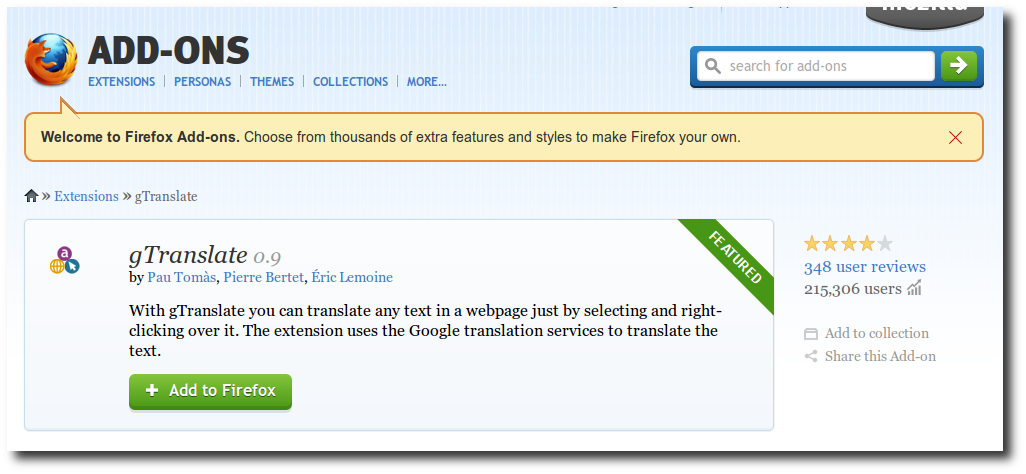
\includegraphics[width=0.8\textwidth]{gtranslate1}
	\index{Firefox!granslate}
\end{figure}

\begin{figure}[h!]
	\centering
	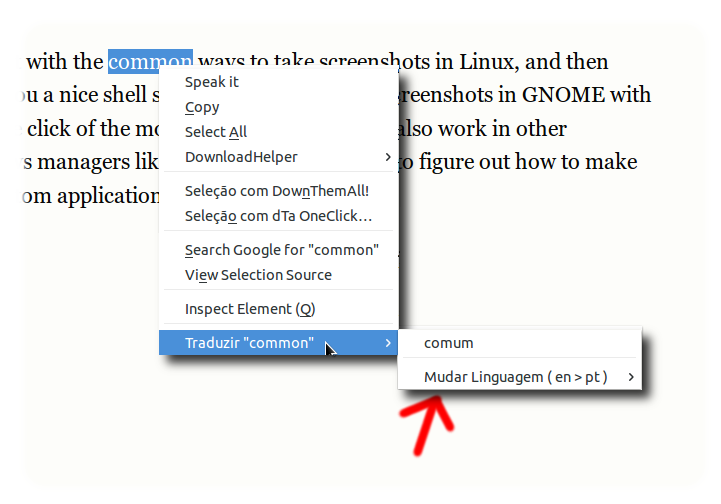
\includegraphics[width=0.8\textwidth]{gtranslate-menu}
\end{figure}

\begin{center}
\noindent
{\footnotesize \ding{42} lembre-se de selecionar o idioma no local indicado.}
\end{center}

\noindent
{\footnotesize \ding{42} Lembre-se que os recursos que mostraremos a seguir só serão melhor aproveitados
se você obtiver um resultado no qual a palavra buscada esteja em um contexto.}

\vspace{0.3\baselineskip}
\noindent
{\footnotesize \ding{42} Na página~\pageref{img:video-helper}, seção \ref{sec:ouca}
descubra como baixar vídeos do youtube}

\newpage
\noindent
Se você digitar no google {\em What does {\bf dig} mean}, ele retornará \dots

\begin{figure}[h!]
	\centering
	\caption {O significado de {\bf dig}}
	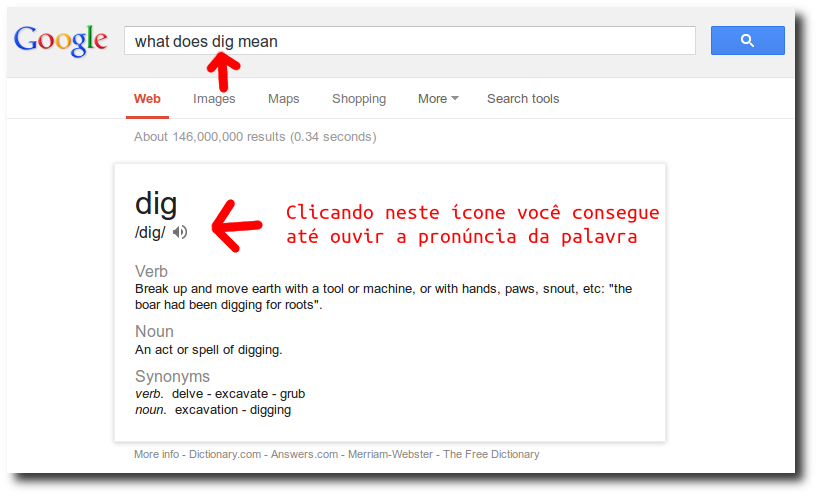
\includegraphics[width=0.8\textwidth]{google}
\end{figure}

\begin{figure}[h!]
	\centering
	\caption{Usando o google tradutor}
	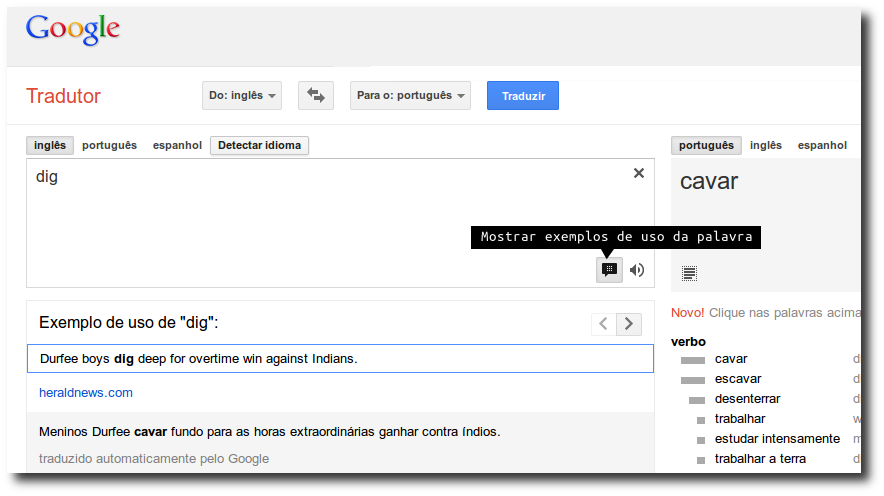
\includegraphics[width=0.8\textwidth]{google-translate}
\end{figure}

\noindent
Na janela do google translate você pode clicar no auto-falante para ouvir
o som em cada idioma bem como clicando sobre a palavra traduzida ele lhe
dá um exemplo contextualizado, clicando sobre o contexto dado ele exibe
a tradução da frase contextualizada.

Do mesmo modo que você pode estudar a gramática de um idioma simplesmente
convivendo com o mesmo, pode também estudar inglês sem pensar diretamente em
estudar inglês, muitas crianças aprendem muitas palavras em inglês simplesmente
porque elas estão presentes nos seus video games.

\section{Como tornar páginas na web mais legíveis}
\index{Firefox!Legibilidade}

Durante seu estudo do inglês você por vezes vai se deparar com um problema
bastante comum, o layout\footnote{a disposição dos caracteres na tela e seu
tamanho na tela} na maioria das vezes dificulta a leitura, neste ponto você está se
deparando com um problema bem diverso do seu foco que é melhorar
seu inglês, o texto está lá, mas a sua legibilidade
está prejudicada, a fim de contornar este problema instale a extensão readability a mesma
pode ser encontrada neste link \href{http://www.readability.com/addons}{http://www.readability.com/addons}.

\begin{figure}[h!]
	\centering
	\caption{{\footnotesize Clique no botão verde}}
	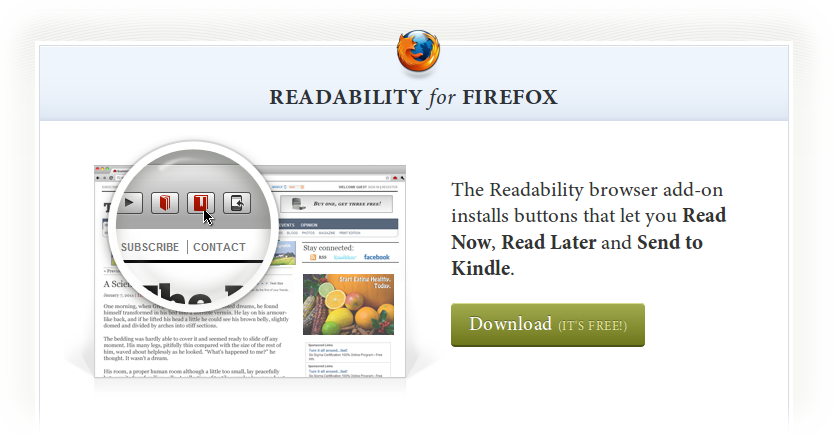
\includegraphics[width=0.8\textwidth]{readability-1}
\end{figure}

\begin{figure}[h!]
	\centering
	\caption{{\footnotesize Texto transformado com o readability}}
	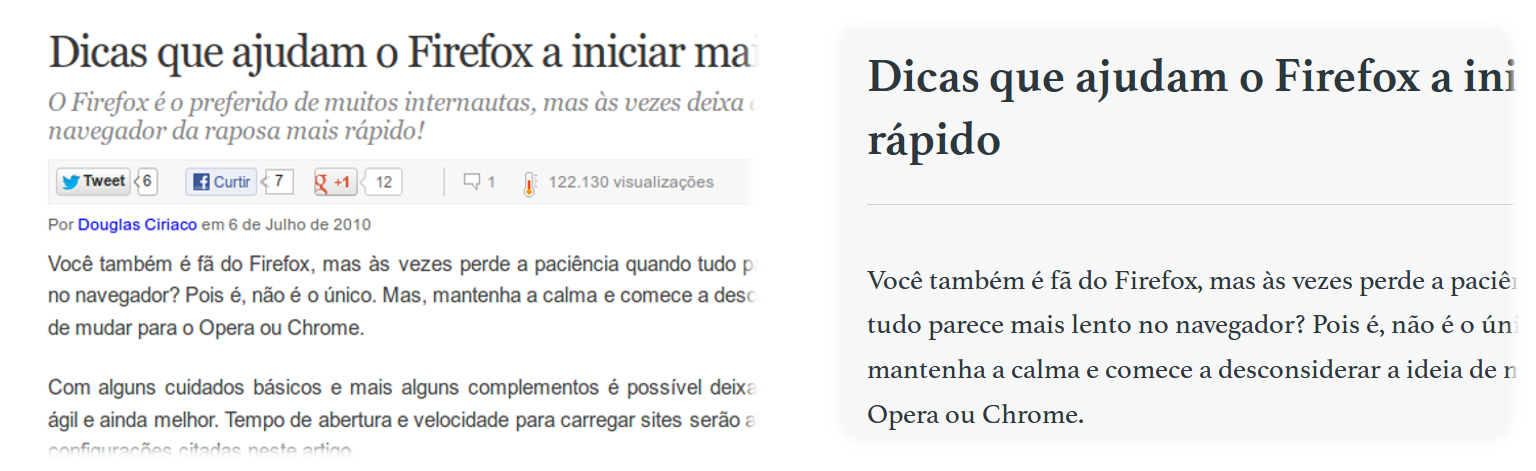
\includegraphics[width=1.2\textwidth]{readability-2}
\end{figure}

\begin{center}
{\footnotesize \ding{42}
Leia sobre o readability aqui: \href{http://tecnoblog.net/35554/ler-texto-sites-como-ebook-reader/}{http://goo.gl/a51mu}\footnote{http://tecnoblog.net/35554/ler-texto-sites-como-ebook-reader/}}
\end{center}



% ------------------------------------------------
%          FILE:  listening.tex
%       CREATED:  Dom 30/Dez/2012 hs 15:59
%   LAST CHANGE:  2013 Mar 28 06:38:22 AM
%        AUTHOR:  Sérgio Luiz Araújo Silva
%          SITE:  http://vivaotux.blogspot.com
%       TWITTER:  @voyeg3r
%         SKYPE:  sergioaraujosilva
% -------------------------------------------------

\chapter{O que você pode ouvir você pode dizer}\label{cha:listening}
\index{Listening}

Desde o início ouça inglês real, desse modo você vai aprender a pronúncia
correta sem que isso seja uma preocupação explícita, se você tiver uma boa
pronúncia significa que você será capaz de discernir melhor os sons dos
falantes nativos do inglês, esse é um dos principais motivos que levam pessoas
que se consideram boas no inglês mas que quando chegam nos EUA ficam
completamente perdidas. O título desta seção foi inspirado em um professor de
inglês chamado \emph{Shane M. Peterson} ou \hypertarget{shane}{coach Shane}
\href{https://twitter.com/coachshane}{@coachshane}, ele atualmente vive na
Coreia do Sul e seu canal no \index{Shane!Youtube}
\href{http://www.youtube.com}{youtube} é:
\href{https://www.youtube.com/user/coachshanesesl}{coachshanesesl} Ele tem
várias séries bem legais para estudantes da lingua inglesa, uma delas chamas-se
\href{https://www.youtube.com/user/dailydictation}{``English
Dictation''}\footnote{https://www.youtube.com/user/dailydictation}, ou ditado
diário de inglês. Do mesmo autor cito a série
\href{ttps://www.youtube.com/user/DailyEasyEnglish}{``DailyEasyEnglish''}\footnote
{https://www.youtube.com/user/DailyEasyEnglish}.

\begin{figure}[h!]
	\centering
	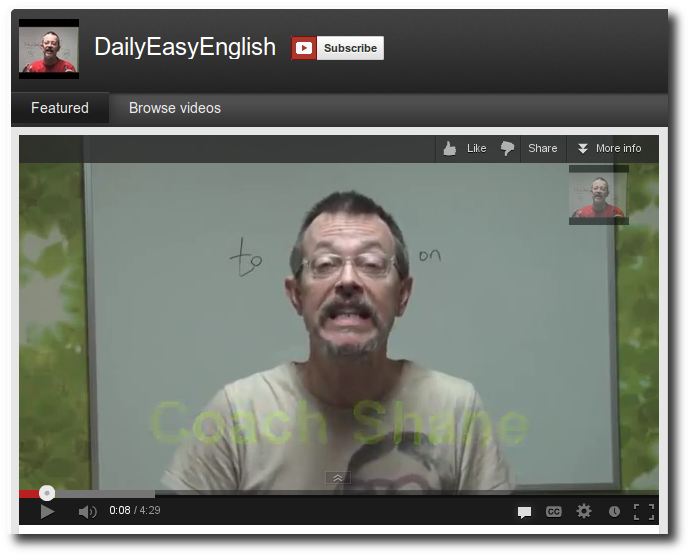
\includegraphics[width=0.8\textwidth]{shane}
	\caption{Coach Shane em uma de suas aulas}
	\index{Shane}
\end{figure}

\noindent Outro professor que tem uma ótima série no youtube é o \index{Teacher
Phill}
\href{https://www.youtube.com/user/TeacherPhilEnglish}{``TeacherPhill''}\footnote{https://www.youtube.com/user/TeacherPhilEnglish}
um de seus canais se chama
\href{https://www.youtube.com/course?list=EC6E296AEDF49E3528}{``Accent Reduction''} e pode ser acessado através deste link:
\href{http://goo.gl/x6SKU}{http://goo.gl/x6SKU} nesta série ele faz a leitura
de um texto e ao final ele fará uma nova leitura mostrando o significado de
algumas palavras e sinônimos.

\vspace{0.3\baselineskip}
\noindent
{\footnotesize \ding{42} ``The great aim of education is not knowledge but action.''
{\em Herbert Spencer} }

\vspace{0.3\baselineskip}
\noindent
{\footnotesize \ding{42} Conheça outros participantes do twitter que postam em inglês na seção
\ref{sec:EnglishLife} página~\pageref{sec:EnglishLife}  }

% tab to continue

\section{Ouça inglês diariamente}\label{sec:ouca}

Ouvir inglês diariamente é uma das principais chaves para atingir a fluência no
inglês, o primeiro passo nessa direção é adquirir um bom
smartphone\footnote{Telefone inteligente} para o qual você deve baixar vários
\index{Podcasts} podcasts e se possível inscreva-se em alguns sites como {\em
twitter} {\em facebook} etc.

Nesta seção você conhecerá alguns links de bons {\em
podcasts}\footnote{Geralmente arquivos em formato mp3 para ouvir em smartphones
e celulares}, ouça inglês pelo menos 30 minutos por dia, para começar um
podcast que é muito bom para iniciantes é o
\href{http://www.eslpod.com/website/index\_new.html}{{\em English as Second Language}}\footnote{http://www.eslpod.com/website/index\_new.html}:
\href{http://goo.gl/Qih6}{http://goo.gl/Qih6} o bom dele é que o audio é lido
pela primeira vez com comentários e de forma bem lenta, certamente você não
compreenderá tudo, mas não se preocupe, em muito pouco tempo você será capaz de
compreende-lo completamente, não tenha tanta pressa.  Outra opção interessante
é o podcast \href{http://edition.englishclub.com/category/listening-news/}{{\em
Listen to the
news}}\footnote{http://edition.englishclub.com/category/listening-news/} no
qual cada audio tem uma transcrição quase completa. Há também um excepcional
podcast intitulado ``culips-english'' que pode ser acessado neste link:
\href{http://esl.culips.com/}{http://esl.culips.com/}, são duas canadenses que
narram histórias muito boas, neste podcast muitas dicas legais, não deixe de
visitar. O site
\href{http://www.bbc.co.uk/portuguese/topicos/aprenda\_ingles/}{``BBC
Brasil''}\footnote{http://www.bbc.co.uk/portuguese/topicos/aprenda\_ingles/}
também tem um acervo bastante interessante neste caso específico você assite
a vídeos nos quais é feita a introdução de novos termos, a história é então
contada e ao final a mesma história é recontada com legendas (Note que
entre os tópicos a serem lidos tem uns com setinhas ``são os vídeos''). Visite
também o site \href{http://www.newsinslowenglish.com/}{\emph{http://www.newsinslowenglish.com/}}.
Neste link do englishclub.com {\footnotesize \ding{42}} \href{http://goo.gl/DkUva}{http://goo.gl/DkUva} você encontrará
dezenas de ditados, ou seja, exercícios para testar
sua capacidade de ouvir.

\vspace{0.3\baselineskip}
\noindent
Um bom canal do \index{VOA!youtube} youtube para quem está começando no inglês
é o \index{VOA} \href{https://www.youtube.com/user/voalearningenglish}{{\em VOA
- Voice of America}}\footnote{https://www.youtube.com/user/voalearningenglish}
pois as notícias lidas nele aparecem com legenda e em 1/3 da
velocidade normal, você pode baixar os videos desse e de outros canais
instalando a extensão video download helper para o firefox à partir deste link:
\href{http://goo.gl/S0xvP}{http://goo.gl/S0xvP} -- {\em link
orignal}\footnote{https://addons.mozilla.org/en-US/firefox/addon/video-downloadhelper}.
\label{Youtube!baixar vídeos} \index{Firefox!video download helper}

\begin{figure}[h!]
	\centering
	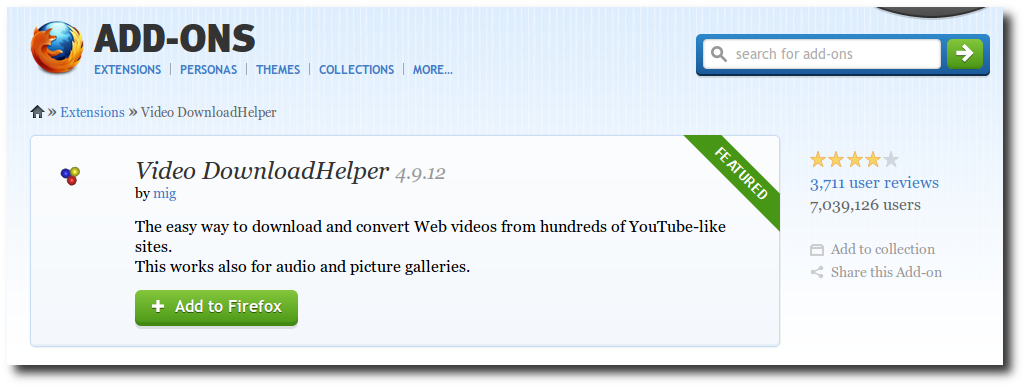
\includegraphics[width=0.8\textwidth]{video-helper}
	\label{img:video-helper}
\end{figure}

\noindent
{\footnotesize \ding{42}  Após instalada a extensão aparecem umas bolinhas coloridas no
lado da barra de endereços do navegador, clicando na setinha ao lado
e escolha a opção ``medium'' que é a de melhor qualidade.}

\vspace{0.3\baselineskip}
\noindent
{\footnotesize \ding{42} Veja também a extensão gtranslate na subseção \ref{sec:google}
na página~\pageref{sec:google}}

\vspace{0.3\baselineskip} \noindent Para usuários Linux há outra opção que permite baixar
playlists do youtube, trata-se do programa
\href{http://rg3.github.com/youtube-dl/}{{\tt
youtube-dl}}\footnote{http://rg3.github.com/youtube-dl/}, no Ubuntu Linux
instale o programa através do comando:\\

{\tt sudo apt-get install youtube-dl \&\& sudo youtube-dl -U}

\vspace{0.3\baselineskip}
\noindent
Para baixar um playlist inteiro faça:\\

{\tt youtube-dl -cit  https://www.youtube.com/user/DailyEasyEnglish}

\section{Como ter vídeos do youtube no celular}
\label{sec:como_ter_v_deos_do_youtube_no_celular}

A extensão \emph{Video Download Helper} citada anteriormente permite baixar
vídeos em formato mp4, \emph{para o caso de aparelhos mais modernos},
mas se você não possui um smartphone, ou seja, tem um celular comum a
extensão lhe permite baixar os vídeos em formato
\emph{3gp}\footnote{https://pt.wikipedia.org/wiki/3GP} , com este
formato você pode ver o vídeo no seu celular, mesmo que ele seja um
aparelho simples.

\begin{figure}[h!]
	\centering
	\caption{Vídeo baixado compatilvel com celulares mais modestos}
	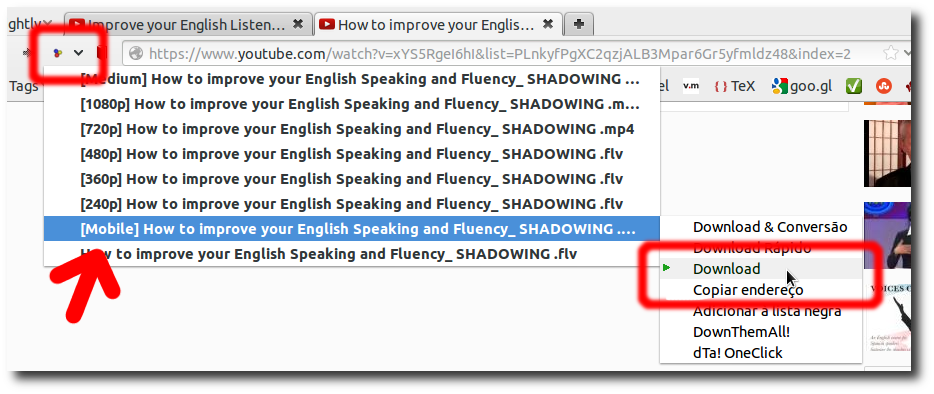
\includegraphics[width=0.8\textwidth]{mobile}
\end{figure}

% section como_ter_v_deos_do_youtube_no_celular (end)

\section{Como melhorar sua capacidade de ouvir}
\label{sec:como_melhorar_sua_capacidade_de_ouvir}

O simples fato de ouvir muito inglês pode não ser suficiente para
garantir uma melhora consistente na sua capacidade de compreensão,
você deve evitar algumas armadilhas. {\footnotesize \ding{42} fonte:
\href{https://www.youtube.com/watch?v=EkxaoaF5wgw}{https://www.youtube.com/watch?v=EkxaoaF5wgw}}.

\begin{description}
	\item[Material muito difícil] e você não entende.
	\item[O material não é interessante para você] e você não se importa.
	\item[É algo chato] e você realmente não quer ouvir.
\end{description}

\dots Se você ouve coisas que tem uma ou mais características acima
é natural que você não se concentre ou absorva o inglês como uma espoja.
Tudo o que você precisa é ouvir conteúdos que são o oposto das características
citadas acima.

\begin{description}
	\item[O material é fácil] e você entende.
	\item[É interessante pra você] e você se importa.
	\item[É excitante] e você quer ouvir.
\end{description}

% section como_melhorar_sua_capacidade_de_ouvir (end)

\section{Os blocos sonoros}\label{sec:blocos-sonoros}

Imagine uma conversação comum do dia-a-dia na qual uma pessoa diz
``você vai mesmo?'', na verdade a palavra {\em você} muitas vezes
transforma-sem em {\em cê} e a palavra {\em mesmo} transforma-se em
{\em mêz}, temos então um grande bloco sonoro, com todos os fonemas
ligados mais ou menos assim: ``cêvaimês.'' No idioma inglês acontece
exatamente a mesma coisa, os sons são abreviados (principalmente
quando se fala rápido) e além disso acontecem as ligações sonoras que
em inglês chamam-se {\em linking words}, {\em reductions} ou ainda
morphing, por exemplo na lingua escrita, ou nos livros formais é comum algo do tipo:
\underline{{\em I wanto to buy a car}}, mas no inglês falado a coisa fica assim:
{\em  \underline{I \textcolor{red}{wanna} buy a car}}. Veja este outro trecho:
\emph{\textcolor{red}{whatcha} thinking?} sua escrita longa em inglês fica assim \emph{What you are thinking?}
Ao trabalhar a audição (listening) trabalhe sempre prestando atenção em como as palavras são
abreviadas e como seus sons estão conectados, isso explica em parte o
fato de estudantes que se consideram avançados no Brasil não
conseguirem se comunicar por exemplo em uma viagem aos Estados Unidos,
é que no seu método de estudo, geralmente baseado na lingua formal não
é visto nada a respeito da sonoridade coloquial, ou seja, do inglês do
dia-a-dia.

\vspace{0.5cm}
{\footnotesize \ding{42}  have a lo\textcolor{red}{t t}o study for the next test.}
\vspace{0.5cm}

\noindent
Existe uma diferença entre a lingua escrita como por exemplo em ``What you do?'',
em relação ao mesmo trecho pronunciado no dia-a-dia ``Wharia do?''
\vspace{0.5cm}

\noindent
Para completar a compreensão dos blocos sonoros o estudante deverá conhecer os
{\em Slangs} que são as gírias, os provérbios e os {\em phrasal verbs}, que são
duas ou mais palavras combinadas que ganham novo sentido devido o contexto em
que se encontram.  Pra finalizar, tenha consciência que você deverá buscar
conversas reais, de falantes nativos, pois a pronúncia e a entonação são
naturalmente corretos. Lembre-se se você conviver com quem tem uma pronúncia
ruin ou não totalmente perfeita você tenderá naturalmente a reproduzir seus
erros. Para aprender mais como combinar palavras veja as lições do
professor \hyperlink{shane}{Shane} no capítulo \ref{cha:listening} página~\pageref{cha:listening}.

\subsubsection{Não estude pronúncia de palavras isoladas}

O contexto também determina a pronúncia de certas palavras, portanto tentar
aprender a pronúncia de palavras isoladas não lhe dará a habilidade de ouvir ou
pronunciar inglês real. Por exemplo a palavra ``to'', em algumas frases ela
muda completamente a sonoridade para algo como: ``I’m going {\bf tuh} the
store.'' \\
{\footnotesize \ding{42}  Para mais detalhes veja:
\href{http://www.englishanyone.com/index.php?page=jsbo3day2}{www.englishanyone.com}\footnote{http://www.englishanyone.com/index.php?page=jsbo3day2}.}

\noindent
{\footnotesize \ding{42} Um bom site para aprimorar sua pronúncia é o \href{http://pt.englishcentral.com}{http://pt.englishcentral.com}}

\section{Lista de podcasts}
\label{sec:lista_de_podcasts}

\begin{verbatim}
http://elllo.org/
http://www.lyricstraining.com/index.php
http://www.listen-to-english.com/
http://www.learnglish.net/
http://www.audiopuzzler.com/index.html
http://www.listen-and-write.com/
http://accent.gmu.edu/index.php (for getting used to different accents)
http://reallifebh.com/real-life-english-esl-podcasts
\end{verbatim}

% section lista_de_podcasts (end)

% Alguns exemplos com frases reais, do dia a dia:
% \begin{verbatin}
% How ya doin?
% What ya doin today
% I ma fa nof baseball
% \end{verbatin}

% ------------------------------------------------
%          FILE:  mudanca.tex
%       CREATED:  Dom 30/Dez/2012 hs 16:00
%   LAST CHANGE:  2013 Apr 02 08:45:03 AM
%        AUTHOR:  Sérgio Luiz Araújo Silva
%          SITE:  http://vivaotux.blogspot.com
%       TWITTER:  @voyeg3r
%         SKYPE:  sergioaraujosilva
% -------------------------------------------------

\chapter{Mudança constante}

Tenha em mente que ao longo do tempo e com a sua evolução, lições que eram
difíceis se tornarão fáceis, já outras que pareciam muito difíceis se tornarão
simples, portanto colecione todos os vídeos e audios que puder. O que funciona hoje não
funcionará amanhã. Uma coisa muito importante é saber que tudo está sujeito a mudanças
esteja preparado para reconhecer quando uma mudança acontecer.
{\em leia um texto a esse respeito na seção~\ref{sec:abelha} página~\pageref{sec:abelha}}.

\noindent
Adquira o habito de ler ou ouvir dicas de outras pessoas que trilharam
o caminho da fluência no Inglês, aliás este livro é uma coleção de dicas
desse tipo. Pessoas que já trilharam o caminho falam sobre o que
funciona melhor. O aprendizado de idiomas está se tornando cada vez mais
uma atividade colaborativa, os velhos métodos estão sendo
questionados, ou seja o mundo está fervilhando de novidades, seja também
um pesquisador.

\section{Motivação e compromisso}

Será que o meu resultado final pode ser afetado pelo modo como encaro
minha atividade? \dots

\vspace{0.3\baselineskip}
\noindent
{\footnotesize \ding{42} ``Language to me is a means to and end. A tool. A vehicle that allows me
 to explore what the world has to offer. This works out great because
 my life is all about exploring and learning. Not language. Language is
 a means to an end''. \href{http://www.davidmansaray.com/language-puzzle}{David Mansaray} }

\vspace{0.3\baselineskip}
\noindent
{\footnotesize \ding{42} Find something else you’re passionate about, combine it
with language and watch your ability to learn language skyrocket. \href{http://www.davidmansaray.com/language-puzzle}{David Mansaray} }
\vspace{0.3\baselineskip}

\noindent
Tenha muito cuidado com a \emph{zona de conforto} ela é um perigo para
qualquer estudante, considere que se seu objetivo é modesto demais
sua determinação virá na mesma proporção. Sonhos pequenos, pequenas
realizações.

\subsection{Os Três pedreiros}
\label{sub:os_tr_s_pedreiros}

Uma vez um vido uma estrada, deparou-se com uma obra
em início de construção. Três pedreiros, com suas ferramentas,
trabalhavam na fundação do que parecia ser um importante projeto. O
viajante, aproximou-se curioso. Perguntou ao primeiro deles o que
estava fazendo. -- Estou sentando tijolos, respondeu
o pedreiro, o homem agradeceu dirigiu-se ao segundo pedreiro e repetiu a
pergunta.

\noindent
-- Estou construindo uma parede.  O viajante queria saber o que seria
aquela construção, agradeceu ao pedreiro e se dirigiu então ao
terceiro pedreiro: -- O que está você fazendo?

\noindent
Este respondeu: -- Estou construindo uma Catedral!

\noindent
Seguindo caminho o viajante observou que os três estavam
fazendo a mesma coisa mas o que mudava era apenas o modo
como cada um deles encarava sua atividade. Moral da história,
\emph{``O modo como encaramos a realidade determina o quão difícil ou
prazeiroso é a realização de nossas atividades''}.

\vspace{0.3\baselineskip}
\noindent
{\footnotesize \ding{42} A atitude mental é a chave para atingir
grandes resultados na vida, pois se você encara sua atividade
como um meio de atingir algo maior essa atividade torna-se prazeirosa.}

% subsection os_tr_s_pedreiros (end)

\subsection{O inglês não como um fim em si}
\label{sub:o_ingl_s_n_o_como_um_fim_em_si}

\noindent
Busque uma fonte inspiradora para estudar inglês, acho que ganhar muita grana
no futuro com a sua melhor qualificação, ter mais qualidade de vida é um bom
começo, mas saiba que se você não tiver uma motivação muito profunda você não
conseguirá manter o mesmo ritmo de estudos. Desenvolva o seu auto didatismo,
não espere soluções prontas. O estudo do inglês deve ser algo prazeiroso,
reflita positivamente acerca de suas pretensões e principalmente crie uma imagem
mental de como sua vida já está mudando e o quanto irá mudar para melhor com
suas conquistas.

\noindent
Pense no inglês como um meio de atingir um objetivo maior, afinal de
contas você estuda inglês não por ele em si, você estuda inglês para
poder viajar para fora do país, para conseguir um emprego melhor etc.

% subsection o_ingl_s_n_o_como_um_fim_em_si (end)

\vspace{0.3\baselineskip}
\noindent
{\footnotesize \ding{42} Lembre-se que o seu nível de compromisso é um dos principais
fatores que irá determinar seu sucesso.}

\vspace{0.3\baselineskip}
\noindent
{\footnotesize \ding{42} Cadastre-se em vários serviços de estudo de idiomas, assim você estará assumindo compromissos
para os quais é mais difícil arranjar desculpas, se você estuda inglês em grupo e tem reuniões periódicas isso
aumenta o seu comprometimento com seu objetivo. Busque no google ``learn english community''.}
% http://www.readability.com/articles/hte7e9hy

\subsubsection{Exemplo de compromisso}

Certa vez uma amiga minha me disse que havia deixado de fumar, ela também
disse isso para todos os familiares e amigos, um dia eu disse a ela, sabe minha amiga
se você não tivesse criado o compromisso sincero de deixar de fumar você não teria
dito para tantas pessoas que iria fazer isso, agora, mesmo que você pense em
desistir da ideia você iria ficar meio sem jeito diante de tantas pessoas, elas
lhe diriam ``Mas você não tinha dito que iria parar de fumar!!.'' Portanto crie
compromisso com suas metas, dentre as quais a de aprender inglês. Quando você
cria um compromisso sincero de realizar algo o universo conspira a seu favor.

\section{Faça do inglês parte de sua vida}\label{sec:EnglishLife}

Siga pessoas que postam frases em inglês no \href{http://www.twitter.com}{twitter} como
\index{Iramara Loiola} \href{http://www.twitter.com/iraloiola}{@iraloiola} \emph{Iramara Loiola} e outras tantas boas fontes
 de inspiração como: \href{http://www.twitter.com/InspireBookClub}{@InspireBookClub},
\href{http://www.twitter.com/RealLifeEng}{@RealLifeEng} etc. Veja por
exemplo a figura abaixo, se você tem o desejo sincero de aprender inglês será
impossível não buscar a tradução.

\begin{figure}[h!]
	\centering
	\caption{\footnotesize Estudando inglês no twitter}
		
\includegraphics[width=0.8\textwidth]{twitter}
	\index{twitter}
\end{figure}

\noindent
Outra forma de incrementar seus estudo é se cadastrar no site
\href{http://www.aprendendoingles.com.br/}{``English for
Reading''}\footnote{http://www.aprendendoingles.com.br/} que passará
a enviar-lhe uma piada em inglês diariamente, basta acessar o link acima
e colocar seu e-mail no campo indicado na base da página. {\em Veja um exemplo}:

\vspace{0.3\baselineskip}
%\hfill
\begin{minipage}[b]{.8\linewidth}

	{\scriptsize
	\noindent
	{\bf Women talk more than men }

	A husband, proving to his wife that women talk more than men, showed her
	a study which indicated that men use on the average only 15,000 words a day,
	whereas women use 30,000 words a day.

	She thought about this for awhile and then told her husband that women use
	twice as many words as men because they have to repeat everything they say.
	He said, "What?"

	\setlist[1]{itemsep=-5pt}
	\begin{itemize}
		\item husband - marido
		\item wife - esposa
		\item talk - falar
		\item show - mostrar
		\item average - média
		\item whereas - ao passo que
		\item think (think, thought, thought) - pensar
		\item awhile - por alguns instantes
		\item twice - duas vezes
	\end{itemize}
	}
\end{minipage} \hfill

\vspace{0.3\baselineskip}
Há também um site muito legal chamado
\href{http://www.tumblr.com}{``tumblr''}\footnote{www.tumblr.com} no qual tem
um canal chamado \href{http://icanread.tumblr.com/}{``i can
read''}\footnote{http://icanread.tumblr.com/} no qual são postadas muitas
frases legais em inglês como esta \dots

%\vspace{0.3\baselineskip}
\begin{figure}[h!]
	\caption{\footnotesize Uma das muitas imagens do {\bf ``i can read''}}
    \centering
		
\includegraphics[width=0.6\textwidth]{tumblr}
	\index{Tumblr}
\end{figure}

\noindent
{\footnotesize \ding{42} Outro site muito bom para praticar a leitura é o quotes love and life
 \href{http://quotesloveandlife.com/}{http://quotesloveandlife.com/} }

\noindent Se você é da área de informática por exemplo pode se cadastrar no
site \href{http://stackoverflow.com}{stackoverflow.com}\footnote{http://stackoverflow.com},
nele temos listas de discussão divididas por assunto, dessa forma você aprende
algo do seu interesse ao mesmo tempo que estuda inglês, e segundo alguns, esta
é uma das melhores formas de se aprender inglês, assim como se pode aprender
gramática sem estar estudando diretamente gramática, com o inglês é a mesma
coisa, veja a imagem abaixo do site stackoverflow.

\begin{figure}[h!]
	\caption{\footnotesize Aprendendo a programar no stackoverflow}
	\centering
		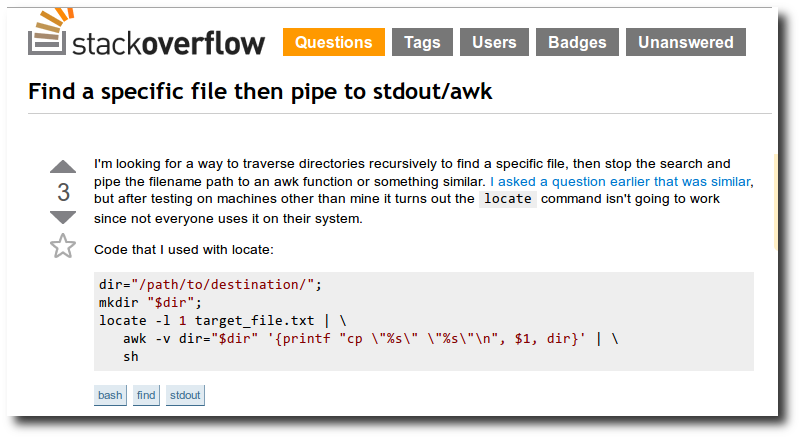
\includegraphics[width=0.8\textwidth]{stackoverflow}
	\label{img:stackoverflow}
\end{figure}

\newpage
\noindent
Configure o seu computador bem como seu smartphone para o idioma
inglês ou qualquer outro que deseje aprender, pode parecer bobagem
mas cada pequeno fragmento de inglês que você aprender faz parte de um
todo, veja um exemplo de uma mensagem do navegador chrome.

\begin{figure}[h!]
	\centering
	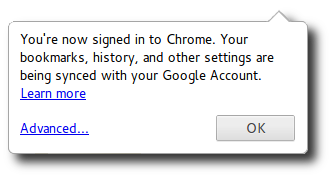
\includegraphics[width=0.8\textwidth]{chrome-browser}
	\caption{chrome-browser}
\end{figure}

\noindent \index{skype}
Um recurso que não pode deixar de ser citado é o \href{http://www.skype.com}{http://www.skype.com} mas
as pessoas tem dificuldades de encontrar parceiros de conversa, para resolver esse problema
O skype tem um link específico para pessoas interessadas em aprender outras línguas o link é este:  \\

\newpage
\href{https://community.skype.com/t5/Language-learning/bd-p/Languages}{https://community.skype.com/t5/Language-learning/bd-p/Languages}

\begin{figure}[h!]
	\centering
	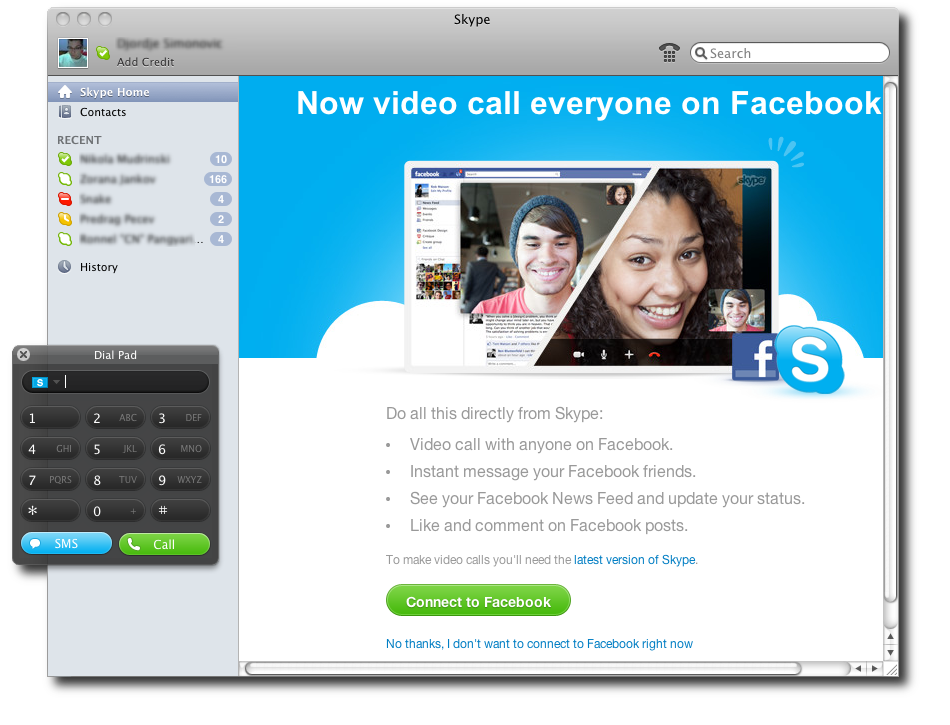
\includegraphics[width=0.8\textwidth]{skype}
	\caption{uma imagem do skype}
\end{figure}

\noindent
O site \href{https://www.verbling.com}{https://www.verbling.com} fornece um serviço parecido com o que é oferecido
pelo skype, contudo ele usa como ferramenta o serviço do google
chamado ``Google Hangouts'', você se cadastra ele pede que você
preencha qual a sua lingua de origem e qual lingua deseja aprender.
Ele oferece dois modos de estudar, um em que ele busca um parceirto da
lingua desejada que deseja aprender sua lingua, e no outro modo você
assiste e/ou entra em um Hangout existente.

\section{Aprenda a digitar}

Volta e meia você precisará de sites tradutores como
o \href{http://translate.google.com}{tradutor do
google}\footnote{http://translate.google.com/} e neles por vezes ao invés de
colar uma frase você terá que digitar, irá se cadastrar no site {\em \href{http://duolingo.com}{Duolingo}},
lá você terá muitas lições nas quais você ouve um audio e terá que digitar
o que ouviu. Outra opção possível é o site
\href{http://www.lingue.pt/}{Linguee}\footnote{http://www.linguee.pt/} no qual
digitamos uma palavra e ele nos mostra a mesma dentro de um contexto.  Se sua
digitação é ruim isso será um impecilho.

\vspace{0.3\baselineskip}
\noindent
{\footnotesize \ding{42}  Um programa livre muito bom para aprender a digitar,
é o \href{http://klavaro.sourceforge.net/pt/index.html}{klavaro}\footnote{http://klavaro.sourceforge.net/pt/index.html}.}

\section{Curso gratuito na Internet}
\index{Duolingo}

Um projeto bastante inovador no aprendizado de idiomas é o \index{Duolingo}
\href{http://duolingo.com}{Duolingo}\footnote{http://duolingo.com} a proposta
é que os usuários aprendam um idioma enquanto ajudam a traduzir artigos
e documentos. Recentemente o {\em Rubens Queiroz de Almeida}\footnote{queiroz@iname.com} o mesmo criador do
{\em livro das 1000 palavras mais comuns do inglês}\footnote{Baixe o livro aqui: http://goo.gl/jbyBZ} publicou no site
Dicas-l da Unicamp um artigo intitulado \href{http://www.dicas-l.com.br/arquivo/colaboracao\_em\_massa\_na\_internet.php}{``Colaboração
em massa na Internet''}\footnote{http://www.dicas-l.com.br/arquivo/colaboracao\_em\_massa\_na\_internet.php}
 falando sobre o projeto Duolingo ele inclusive traduziu um vídeo inteiro no qual um dos criadores
do Duolingo fala como surgiu a ideia do mesmo.

%\vspace{0.3\baselineskip}
\begin{figure}[h!]
	\centering
	\caption{Captura de tela do site {\em Duolingo}}
	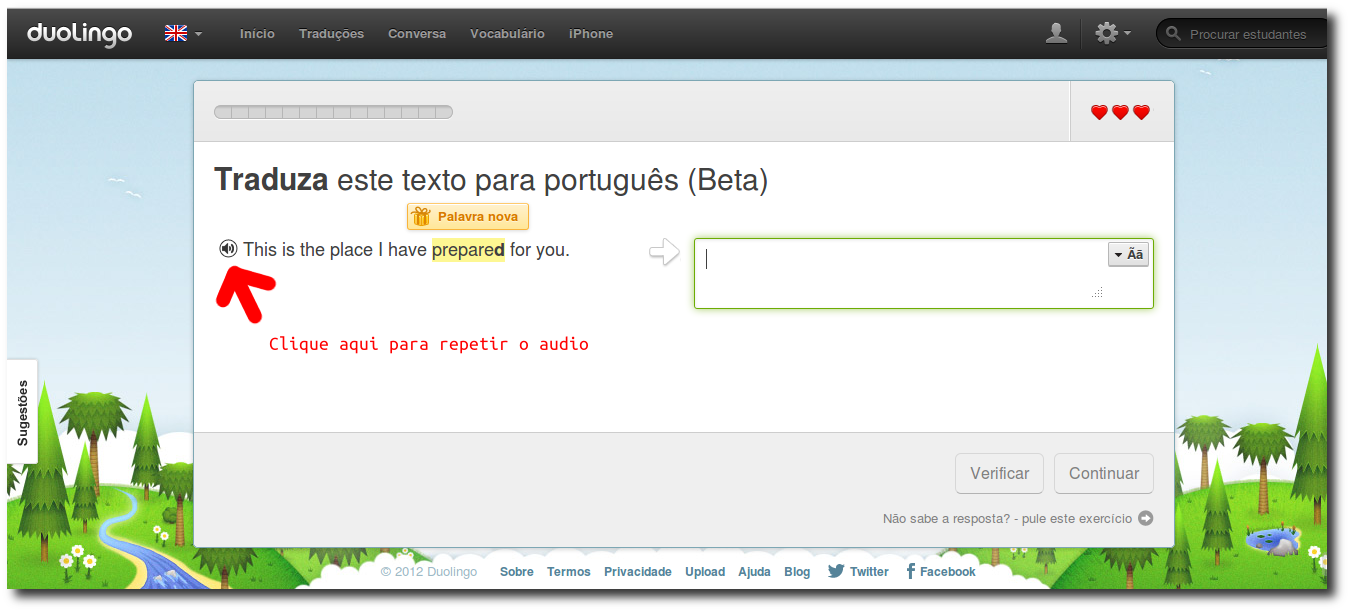
\includegraphics[width=0.8\textwidth]{duolingo} \\
\end{figure}

\begin{figure}[h!]
	\centering
	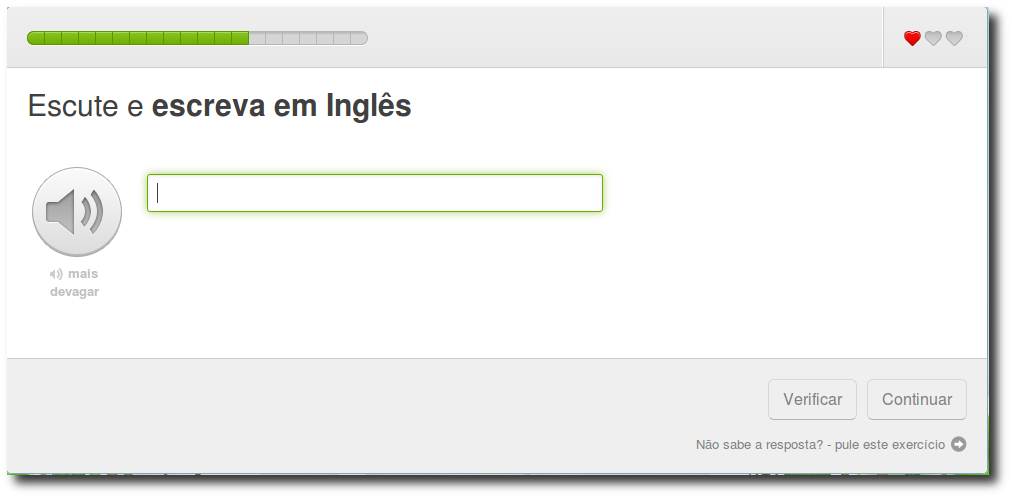
\includegraphics[width=0.8\textwidth]{duolingo-2}
\end{figure}

\vspace{0.3\baselineskip}
{\footnotesize \ding{42}  Há também uma versão do duolingo para Android\footnote{Smartphone do google}}

\section{Leia e escreva em inglês constantemente}
\label{sec:leia_e_escreva_em_ingl_s_constantemente}

Ao ler e escrever você aumentará seu vocabulário constantemente,
quando você formula novas frases vez por outra terá que buscar
palavras que ajudem na contrução de ideias. Durante a leitura proceda
a mesma em voz alta para melhorar sua pronúncia, ao mesmo tempo em que
surgirão constantemente palavras novas, marque-as e busque no site
\href{http://linguee.com}{http://linguee.com} frases contendo a
palavra em questão, anote as frases em formato de \emph{Flashcards}.
(veja mais sobre os Flashcards na
seção~\ref{sub:programas_para_memoria_o}
página\pageref{sub:programas_para_memoria_o})  São retângulos em
cartolina em que de um lado está a frase em inglês e do outro a sua
tradução.

Existe um site chamado \href{http://lang-8.com/}{http://lang-8.com/}
no qual os textos que você envia serão corrigidos por nativos da
lingua alvo e você poderá ajudar pessoas que desejam aprender
português, assim você controi aos poucos um círculo de amizades em que
a ajuda mútua é a tônica.

% section leia_e_escreva_em_ingl_s_constantemente (end)

\section{Crie um livro de anotações}\label{sec:evernote}
\index{Evernote}

Crie um livro de anotações no qual você anota frases nas quais aparecem
palavras novas, isto é necessário pelo fato de que novas palavras se não
anotadas são dificilmente memorizadas, a revisão periódica das anotações
garante o aprendizado. Outra possibilidade é criar uma conta no site
\href{https://evernote.com/}{evernote}\footnote{https://evernote.com/} no qual
você pode salvar artigos inteiros para consultas posteriores. A grande vantagem
de ter uma espécie de bloco de notas online é que independente de onde você
esteja, seja em casa, no trabalho ou durante uma viagem o seu conteúdo está
acessível.  Também fortemente recomendado é a criação de uma conta no site de
favoritos online
\href{https://www.delicious.com/}{delicious}\footnote{https://www.delicious.com/}.
Normalmente as pessoas usam os favoritos do navegador, contudo as páginas que
você salva estão geralmente no computador de casa, quando você chega no
trabalho os favoritos de casa não estão mais acessíveis e vice-versa, com
o {\em delicious} seus favoritos estão em qualquer lugar em que exista acesso
a web.

\vspace{0.3\baselineskip}
\noindent
{\footnotesize \ding{42}  Há uma versão do {\em evernote} para {\em Android}}

\vspace{0.3\baselineskip}
\noindent
{\footnotesize \ding{42} There is no growth without change, no change without fear or loss, and no loss
without pain. http://simurl.com/zobbaj  pg 220 }

\vspace{0.3\baselineskip}
\noindent
{\footnotesize \ding{42} this section brings to you one gift :) \href{http://www.ecenglish.com/learnenglish/}{http://www.ecenglish.com/learnenglish/} }


% ------------------------------------------------
%          FILE:  salto-quantico.tex
%       CREATED:  Dom 30/Dez/2012 hs 15:58
%   LAST CHANGE:  2013 Mar 27 08:35:47 PM
%        AUTHOR:  Sérgio Luiz Araújo Silva
%          SITE:  http://vivaotux.blogspot.com
%       TWITTER:  @voyeg3r
%         SKYPE:  sergioaraujosilva
% -------------------------------------------------

\chapter{O salto quântico do aprendizado}\label{salto-quantico}
\index{Salto quântico}

\section{Nem sempre o difícil é o certo}\label{sec:abelha}
\index{Fluencia}

{\footnotesize from: Fluência em inglês \dots -- \href{http://goo.gl/CcuIk}{Fluency Academy no Facebook}\footnote{http://goo.gl/CcuIk}}

\dots Eu estava na sala de estar de minha casa. É um lugar pacífico com visão
para o lago Kootenay na pequena montanha de Nelson, British Columbia, Canadá.
Passava de meio dia, no final de junho, e eu estava testemunhando uma luta de
vida e morte a apenas alguns passos de distancia. Na sala, comigo, estava uma
grande abelha, que estava presa na casa, e tentando sair, ela estava usando
todas as suas forças tentando voar através do vidro janela da sala de estar.
Repetidas vezes, suas asas zumbiram intensamente, a abelha desesperada se
jogava no vidro da janela. A estratégia da abelha para escapar era fácil de
perceber -- ``tentar com força'' (try harder). Claramente esta estratégia não
estava funcionando! No outro lado da sala, dez passos de distancia, a porta de
traz da casa estava estava aberta, dez segundos de voo e a ``embaraçada
abelha'' poderia alcançar a liberdade. Com apenas um pouco de esforço, e uma
pequena parcela de coragem de voar através do ``desconhecido'', a abelha
poderia facilmente se libertar alcançando seu objetivo que era ir para o lado
de fora. A possibilidade de descoberta está lá. Uma simples mudança em seu modo
de agir irá trazer o resultado desejado, isto pode ser fácil! Porque a abelha
não tentou outro método? Porque ela continuou com seu método quando claramente
ele não estava funcionando? Muitas vezes nós todos ficamos ofuscados ``tentando
duro'', com métodos que não parecem funcionar. Isto parece ser especialmente
verdade quando se trata de nossa habilidade no idioma inglês.

Mas ``tentando duro'' para desenvolver a habilidade de se comunicar
e a confiança não é necessariamente o melhor método para alcançar seu objetivo
de falar com confiança o inglês fluente. Algumas vezes, de fato, a estratégia
do ``Trabalho duro'' é em grande parte do problema que impede você de alcançar
seu objetivo.

\section{O que é um salto quântico?}
\index{Salto quântico!O que é salto quântico}
% fazer referência ao conteúdo quantum leap
O salto quântico é uma palavra tomada do vocabulário da nova Física - A Física
Quântica é a ciência que ajudou-nos a ter a televisão, computadores,
comunicação via satélite e energia nuclear. A Física Quântica tem sido descrita
como a mais poderosa ciência que a humanidade jamais descobriu. E ela requer
que nós repensemos as ideias que nós temos sobre tempo e espaço, e como
a consciência humana trabalha.

A Física Quântica também tem coisas incríveis para dizer sobre você, seu
potencial, e o poder da mente. Para simplificar, como seres humanos nós teremos
que reexaminar nossas ideias de como o universo trabalha e como nós nos
encaixamos nele. {\em Margaret J. Wheatley}, em seu premiado livro, ``Liderança
e a Nova Ciência'', descreve um salto quântico como:

\begin{quotation}
\noindent
``\dots Quando um elétron pula de uma órbita para outra sem passar através de estágios
intermediários. Está em um lugar e repentinamente em outro.''
\end{quotation}

Os Físicos que estudam o a ciência quântica tem notado que os elétrons fazem
estes ``saltos'' de um nível para outro nível vários estágios acima \dots\ sem
nenhum real esforço, e sem ir passo-a-passo do ponto de partida para
o ponto de chegada. O que está acontecendo aqui? Porquê isto acontece?
E é possível para você como um indivíduo dar um `salto' tão grande e sem esforço em
suas habilidades de comunicação em inglês e nível de confiança? É possível para você fazer
o Salto Quântico no Inglês?

\newpage
\section{A estratégia do Salto Quântico}\label{sec:estrategia}
\index{Salto quântico!Estratégia}

A estratégia do salto quântico, segundo Daniel E. Cotton baseia-se
na ideia de que você como indivíduo pode experimentar um salto quântico
no aprendizado, ou seja, pode alcançar um nível vários estágios acima, para
isso ele desenvolveu o que chama fluency framework, o mesmo tem alguns princípios:

\vspace{0.3\baselineskip}
\noindent {\bf As armadilhas do aprendizado} \\
Existem seis armadilhas que lhe impedem de chegar a sua fluência:
\begin{description}
	\item [Be reasonable]: Ser moderado em suas pretensões e expectativas, ou seja pensar pequeno.
		\item [More the same]: o método que lhe trouxe até este nível foi útil mas ele não lhe levará aos próximos níveis,
			isto se baseia na afirmação de Einstein:\\ {\footnotesize \ding{42} ``Insanity: doing the same thing over and over again and expecting different results'' }.
		\item [Play it safe]: O medo de correr riscos, especialmente de cometer erros ou de tentar algo novo como
			no caso da abelha na seção \ref{sec:abelha} página~\pageref{sec:abelha}.
		\item [Do it alone]: Baseia-se no livro ``O Segredo'', em que o universo conspira a seu favor, por exemplo:
			dizendo para muitas pessoas que está estudando inglês você cria compromisso.
		\item [Disengaged heart]: Se você acredita ser capaz você busca e acha os meios, se você não se acha capaz
			você não tem o mesmo entusiasmo e para no meio do caminho.
		\item [ Need more preparation]: Segundo Daniel E. Cotton a maioria das pessoas já possuiu
			o vocabulário necessário para ser fluente, veja a seção {\em Completando frases} na página \pageref{sub:frases}.
\end{description}

\noindent
Também segundo Daniel E. Cotton {\em Phrasal Verbs, Idioms, Linking Words, vocabulário etc.} fazem parte do que ele chama
de parte mecânica do aprendizado, a parte psicológica involve os pontos citados nas armadilhas do aprendizado, devemos concentrar
80\% do esforço na parte psicológica e apenas 20\% na parte mecânica.

\vspace{0.3\baselineskip}
{\footnotesize \ding{42} ``The reasonable man adapts himself to the world; the unreasonable one persists
in trying to adapt the world to himself.
Therefore, all progress depends on the unreasonable man.'' \\
                                 -- George Bernard Shaw}

\subsection{Completando frases}\label{sub:frases}

Neste ponto, muitos estudantes de inglês com os quais falo dirão: ``Este é um
grande método Daniel\footnote{Daniel E. Cotton}, mas eu não sei como fazer.''
Para estes estudantes, eu respondo gentilmente, ``Sim, na verdade você sabe.
Todas as respostas que você necessita estão na sua mente. Você necessita apenas
fazer as perguntas certas.'' Então, para provar-lhes isto, eu frequentemente
lhes dou uma atividade de complementação de sentenças, eu escrevo ou digo
o começo de uma sentença, e os deixo finaliza-la. Por exemplo, eu inicia
a seguinte sentença: \vspace{0.3\baselineskip}

``Somo things I can do now to improve my English communication skills are \dots''
\vspace{0.3\baselineskip}

É incrível o quão rápido eles conseguem completar as sentenças. Eles imediatamente dirão \dots

\setlist[1]{itemsep=-4pt}
\begin{itemize}
		\item Take an English speaking colleague out to lunch
		\item Find an online English instructor to work with
        \item Model great English speakers and presenters
        \item Form an English Master Mind group with like-minded professionals
        \item etc \dots
\end{itemize}

A maioria dos estudantes ficam surpresos em o quão rapidamente eles podem
completar a atividade de complementação de sentença. Eles sentem um novo senso
de confiança quando se dão conta de que já tem a respostas dentro deles.

Eu vou dar a você atividades de complementação de sentenças neste livro, eu
os chamo de {\em fundamentos de fluência}. Finalize cada uma das sentenças com
várias respostas. Seja honesto o quanto possível
sem parar para pensar muito sobre a mesma. Não se preocupe se o final faz ou
não sentido, se é profunda ou mesmo se é verdadeira. Simplesmente escreva o que
vier a sua mente \dots \hspace{0.3\baselineskip} \dots  mas escreva algo.

When you complete these simple yet profound statements, you will start to
immediately experience a shift in your thinking and actions. You will
experience a Quantum English Leap!

Quando você completar estas simples mas profundas afirmações, você imediatamente
começará a experimentar uma mudança em seu modo de pensar e em suas ações. Você
experimentará o salto quântico no inglês! Você irá experimentar o salto quântico
do aprendizado do inglês.

\vspace{0.3\baselineskip}
\noindent
Complete the following sentence using only {\bf one} or {\bf two} words:\\
Fluency is \dots

\vspace{0.3\baselineskip}

\noindent
Fill in the blank: \newline
Yesterday, I read \dots ? pages in English.

\vspace{0.3\baselineskip}
\noindent
Complete the sentences below: \\
1. One thing about my English that I am {\bf proud} about right now is \dots \newline
2. One thing about my English that I am {\bf grateful} for right now is \dots \newline
3. One thing about my English that makes me {\em excited} right now is \dots \newline
4. One thing about my English that I am {\bf committed} to right now is \dots \newline
\newline
Question: \newline
\noindent
What do {\bf you} do to raise your `competence' in English? \newline
What do {\bf you} you do become a more `proficient' English speaker? \newline
What do {\bf you} you to do to speak English more correctly? More accurately? \newline

\noindent É interessante notar que a proposta do ``salto quântico do
aprendizado'' engloba a ideia de {\em não estudar palavras isoladas} vista na seção
\ref{sub:aprenda-contextualmente} página \pageref{sub:aprenda-contextualmente},
assim como a ideia dos {\em blocos sonoros} vista na seção \ref{sec:blocos-sonoros}
na página \pageref{sec:blocos-sonoros}.

\begin{multicols}{2}
{\footnotesize
``Every hour I’m [learning a language] feels like a minute. Every minute I am
away from [the language I'm learning] feels like an hour.''

``\dots\ And that is the secret to how to become a polyglot in minutes, not
hours, months, or years. It’s to absolutely love it, so that studying isn’t
a chore; it isn’t a task you want to get out of the way so that you can reach
that fluency you lust for. No, lust fizzles – but if you love the language, if
you love the language-learning process, those hours, those months, and those
years, they’ll fly by.''

\vspace{0.3\baselineskip}
\noindent
The above quote is from (jump to 8’10” in the video) and this post was inspired
by Anthony Lauder from FluentCzech‘s YouTube video entitled Become a Polyglot
in Minutes not Years, which you can view here: \href{http://goo.gl/IB7Hf}{http://goo.gl/IB7Hf} on youtube

\noindent
source: \href{http://mandarinfromscratch.com/2011/06/}{link.}}
\vfill \columnbreak

{\footnotesize
``Toda hora que eu estou [aprendizagem de uma língua] parece um minuto. Cada
minuto que eu estou longe de [a língua que estou aprendendo] parece uma hora.''

``\dots\  E esse é o segredo de como se tornar um poliglota em minutos, não em
horas, meses ou anos. É absolutamente amor, de modo que o estudo não é uma
tarefa, não é uma tarefa que você quer sair do caminho para que você possa
chegar a essa fluência que você ansiar. Não, luxúria fizzles - mas se você ama
a língua, se você ama o processo de aprendizagem da língua, as horas, os meses
e os anos, eles vão voar.''

\vspace{0.3\baselineskip}
\noindent
A citação acima é de (ir para 8'10 "no vídeo) e este post foi inspirado
por Anthony Lauder do vídeo no YouTube intitulado FluentCzech Torne-se um poliglota
em minutos, não anos, que você pode ver aqui: \href{http://goo.gl/IB7Hf}{no youtube}

\noindent
fonte: \href{http://mandarinfromscratch.com/2011/06/}{link}}
\end{multicols}

% ------------------------------------------------
%          FILE:  quantum-leap.tex
%       CREATED:  Dom 30/Dez/2012 hs 16:18
%   LAST CHANGE:  2013 Mar 25 09:05:26 AM
%        AUTHOR:  Sérgio Luiz Araújo Silva
%          SITE:  http://vivaotux.blogspot.com
%       TWITTER:  @voyeg3r
%         SKYPE:  sergioaraujosilva
% -------------------------------------------------

When talking with others in English, never be afraid or shy to ask for
clarification if you don't understand what they said.  Here are a few {\em useful phrases} you can use: \\
{\scriptsize
\noindent
1 - Could you please say that [again, more slowly, in other words, in another way]. \\
2 - I'm sorry, I didn't [hear, understand, catch] that. Could you please [repeat, clarify, rephrase] it. \\
3 - What you just said isn't clear to me \\
e. Could you please go over it one more time? \\
4 - Would you please [explain, tell me] that again? \\
5 - I think I understand what you are saying. Can I repeat it back to you to make sure? \\
}

When using these phrases in conversation; straighten up, make eye contact, show sincerity, and speak slowly and clearly.
Asking for clarification is not something to be embarrassed about. It shows that you care, want to understand


% ------------------------------------------------
%          FILE:  have-fun.tex
%       CREATED:  Dom seg 25 março de 2013 hs 9h
%   LAST CHANGE:  2013 Apr 06 03:48:23 PM
%        AUTHOR:  Sérgio Luiz Araújo Silva
%          SITE:  http://vivaotux.blogspot.com
%       TWITTER:  @voyeg3r
%         SKYPE:  sergioaraujosilva
% -------------------------------------------------

\chapter{Divirta-se ao aprender}

Colecione imagens engraçadas que contenham frases em inglês, piadas,
frases de efeito isso aumentará sua motivação para o estudo.

\begin{figure}[h!]
	\centering
	
\includegraphics[width=0.8\textwidth]{dna}
	\caption{dna}
\end{figure}

\vspace{0.3\baselineskip}
\noindent
{\footnotesize \ding{42} Hear a piece of information and three days later you will remember 10\% of it
 add a picture and you will remember 65\% -- Jonh Medina }

\section{Lista de video chats}
\label{sec:lista_de_video_chats}

Segue uma lista de sites em que podemos bater papo por vídeo, seja
cauteloso pois em alguns deles não há censura, sabendo disso faça suas
escolhas e boa diversão:

\begin{verbatim}
	http://www.tinychat.com/
	http://omegle.com/
	http://www.6rounds.com/
	http://www.tokbox.com
	http://www.anybodyoutthere.com/
	http://www.ekko.tv/
	http://www.palbee.com/
	http://vawkr.com/
	http://www.mebeam.com/
	http://chatroulette.com/
\end{verbatim}

\vspace{0.3\baselineskip}
\noindent
{\footnotesize \ding{42} ``The future belongs to those who believe in the beauty of their dreams''.  Eleanor Roosevelt  }


% section lista_de_video_chats (end)

\section{Ted Talks}
\label{sec:ted_talks}

Que tal aprender inglês assistindo excepcionais palestras com ou sem
legendas o nome do site é Ted Talks e o endereço é este:  \href{http://www.ted.com}{http://www.ted.com}

\begin{figure}[h!]
	\centering
	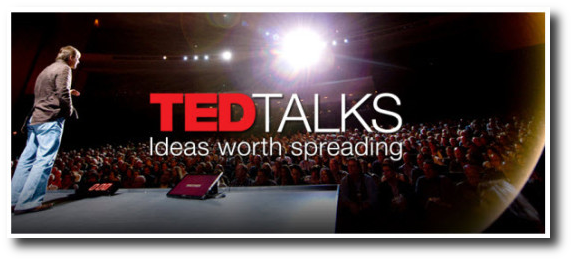
\includegraphics[width=0.8\textwidth]{ted-talks}
	\caption{ted-talks}
\end{figure}

TED (acrônimo para Technology, Entertainment, Design; Tecnologia,
Entretenimento, Design em português) é uma fundação privada sem fins
lucrativos dos Estados Unidos mais conhecida por suas conferências na
Europa, Ásia e Estados Unidos destinadas à disseminação de ideias.
Segundo as palavras da própria organização, “ideias que valem serem
disseminadas”.  As apresentações de Ted Talks são limitadas a dezoito
minutos, e os vídeos são amplamente divulgados na Internet.

O grupo foi fundado em 1984, e a primeira conferência Ted talks
aconteceu em 1990. Originalmente influenciada pelo Vale do Silício,
sua ênfase era tecnologia e design, mas com o aumento da popularidade
os temas abordados passaram a ser mais amplos, abrangendo quase todos
os aspectos de ciência e cultura. Entre os palestrantes no Ted talks
estão Bill Clinton, Al Gore, Gordon Brown, Richard Dawkins, Bill
Gates, os fundadores da Google, Billy Graham e diversos ganhadores do
Prêmio Nobel. Referência:
\href{http://www.hirondino.com/ted-talks/}{http://www.hirondino.com/ted-talks/}

O site disponibiliza links para baixar cada palestra permitindo ainda
selecionar como será a legenda e a qualidade do material baixado. uma
palestra recomendada fala sobre a febre do Inglês ao redor do mundo:
\href{http://goo.gl/bdwUJ}{http://goo.gl/bdwUJ}

% section ted_talks (end)


\printindex

\end{document}

